%%%%%%%%%%%%%%%%%%%%%%%%%%%%%%%%%%%%%%%%%%%%%%%%%%%
\begin{frame}
  \begin{center}
    {\Large Concepts}

  \end{center}
\end{frame}

%%%%%%%%%%%%%%%%%%%%%%%%%%%%%%%%%%%%%%%%%%%%%%%%%%%
\begin{frame}
  \begin{center}
    {\Large Test-case: Classification}

  \end{center}
\end{frame}

%%%%%%%%%%%%%%%%%%%%%%%%%%%%%%%%%%%%%%%%%%%%%%%%%%%
\begin{frame}[fragile] \frametitle{Classify the Data}
Example:
\begin{itemize}
\item Goal: To split the data
\item Try some lines. 
\item Find mis-classification error. 
\item Minimize by Gradient Descent.
\end{itemize}
\begin{center}
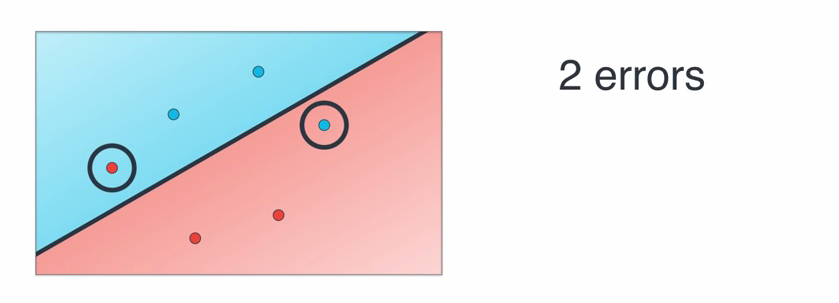
\includegraphics[width=0.8\linewidth,keepaspectratio]{dl1}
\end{center}
{\tiny (Image Credit: A friendly introduction to Deep Learning and Neural Networks -  Luis Serrano)}

\end{frame}

%%%%%%%%%%%%%%%%%%%%%%%%%%%%%%%%%%%%%%%%%%%%%%%%%%%
\begin{frame}[fragile] \frametitle{Error}
\begin{itemize}
\item Problem: Error can be continuous (float) or discrete(int), say number of mis-classifications.
\item But Gradient Descent works only on continuous functions, not on steps!!
\end{itemize}
\begin{center}
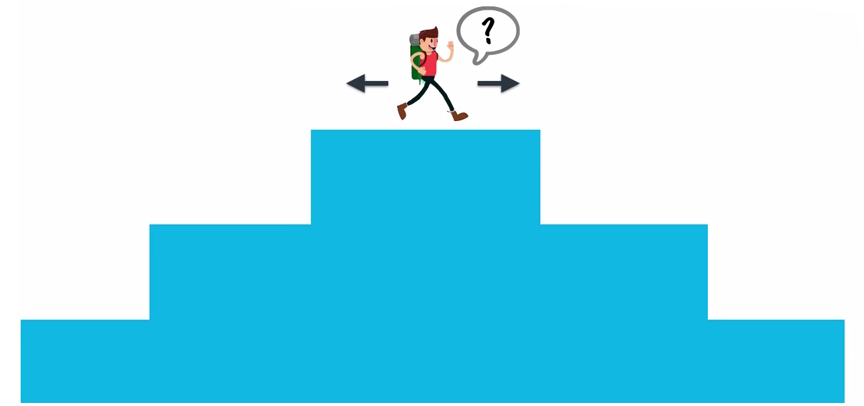
\includegraphics[width=0.7\linewidth,keepaspectratio]{dl2}
\end{center}
{\tiny (Image Credit: A friendly introduction to Deep Learning and Neural Networks -  Luis Serrano)}
\end{frame}

%%%%%%%%%%%%%%%%%%%%%%%%%%%%%%%%%%%%%%%%%%%%%%%%%%%
\begin{frame}[fragile] \frametitle{Penalty}
\begin{itemize}
\item Mis-classified points get more penalty.
\item Error function adds them together. That's a float value.
\item So Error has changed from number of mis-classifications (int) to penalty (float)
\item Penalty makes Error function continuous and thus Gradient Decent can apply.
\end{itemize}
\begin{center}
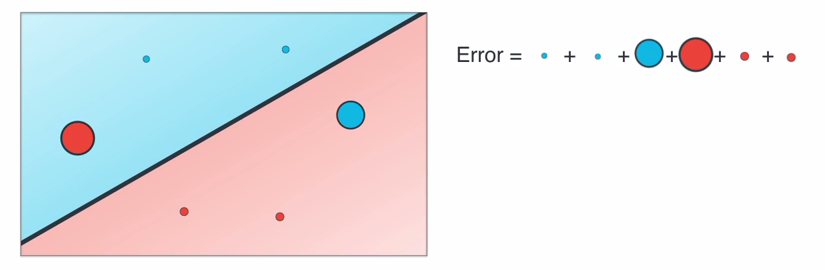
\includegraphics[width=0.7\linewidth,keepaspectratio]{dl3}
\end{center}
{\tiny (Image Credit: A friendly introduction to Deep Learning and Neural Networks -  Luis Serrano)}
\end{frame}

%%%%%%%%%%%%%%%%%%%%%%%%%%%%%%%%%%%%%%%%%%%%%%%%%%%
\begin{frame}[fragile] \frametitle{Activation}
How?
\begin{itemize}
\item Penalty is actually somewhat in the form of Probability
\item See Heatmap of probability.
\item Color intensity is continuous (float)
\item That's Sigmoid. The activation function.
\end{itemize}
\begin{center}
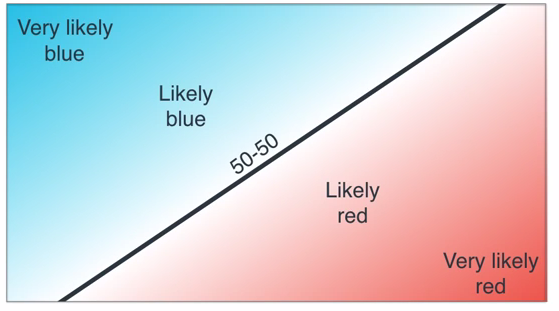
\includegraphics[width=0.7\linewidth,keepaspectratio]{dl4}
\end{center}
{\tiny (Image Credit: A friendly introduction to Deep Learning and Neural Networks -  Luis Serrano)}
\end{frame}

%%%%%%%%%%%%%%%%%%%%%%%%%%%%%%%%%%%%%%%%%%%%%%%%%%%
\begin{frame}[fragile] \frametitle{Likelihood}
\begin{itemize}
\item Sigmoid takes any number, maps it to 0 to 1.
\item Each point thus gets a probability
\item Likelihood of good classification is multiplication of all those probabilities (being independent)
\end{itemize}
\begin{center}
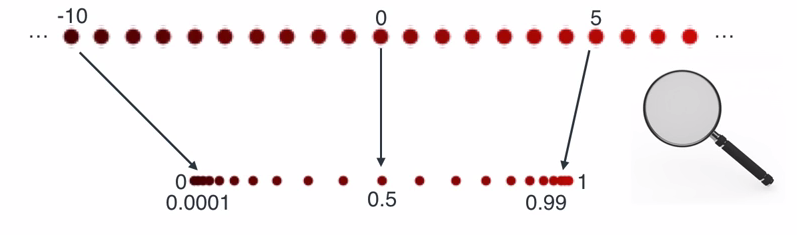
\includegraphics[width=0.7\linewidth,keepaspectratio]{dl5}

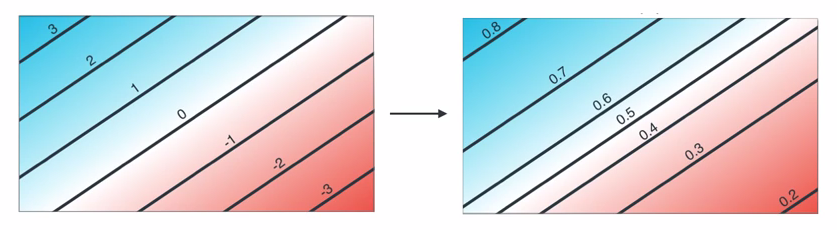
\includegraphics[width=0.7\linewidth,keepaspectratio]{dl6}
\end{center}
{\tiny (Image Credit: A friendly introduction to Deep Learning and Neural Networks -  Luis Serrano)}
\end{frame}


% %%%%%%%%%%%%%%%%%%%%%%%%%%%%%%%%%%%%%%%%%%%%%%%%%%%
% \begin{frame}[fragile] \frametitle{Maximum Likelihood}
% \begin{itemize}
% \item Find the configuration with Maximum Likelihood
% \item Product is converted to sum by log. -ve its as numbers are below 1.
% \item So, Error is summation of all -ve log of probabilities of individual points.
% \end{itemize}
% \begin{center}
% 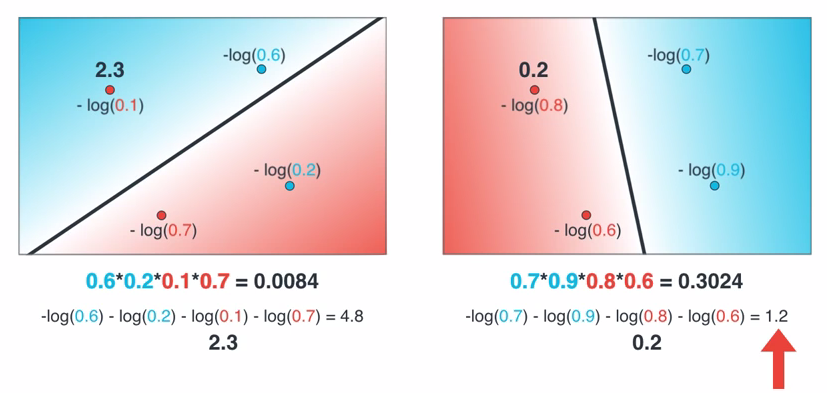
\includegraphics[width=0.7\linewidth,keepaspectratio]{dl7}
% \end{center}
% {\tiny (Image Credit: A friendly introduction to Deep Learning and Neural Networks -  Luis Serrano)}
% \end{frame}

%%%%%%%%%%%%%%%%%%%%%%%%%%%%%%%%%%%%%%%%%%%%%%%%%%%
\begin{frame}[fragile] \frametitle{Maximum Likelihood}
\begin{itemize}
\item Find the configuration with Maximum Likelihood
\item Product is converted to sum by log. -ve its as numbers are below 1.
\item So, Error is summation of all -ve log of probabilities of individual points.
\item Misclassificaitin gets error as 2.3 and the good seen gets 1.2
\end{itemize}
\begin{center}
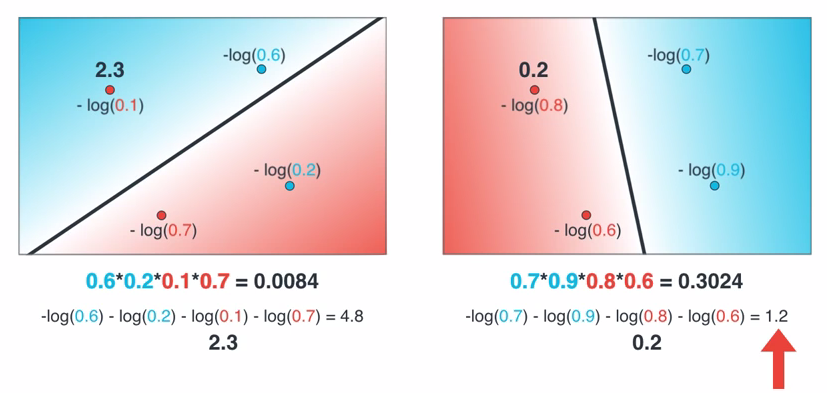
\includegraphics[width=0.7\linewidth,keepaspectratio]{dl7}
\end{center}
{\tiny (Image Credit: A friendly introduction to Deep Learning and Neural Networks -  Luis Serrano)}
\end{frame}

%%%%%%%%%%%%%%%%%%%%%%%%%%%%%%%%%%%%%%%%%%%%%%%%%%%
\begin{frame}[fragile] \frametitle{Logistic Regression}
\begin{itemize}
\item That's all the Logistic Regression.
\item The Eqn of line can be represented as neuron.
\end{itemize}
\begin{center}
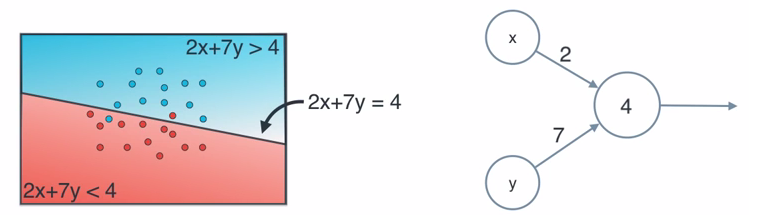
\includegraphics[width=\linewidth,keepaspectratio]{dl8}
\end{center}
{\tiny (Image Credit: A friendly introduction to Deep Learning and Neural Networks -  Luis Serrano)}
\end{frame}

%%%%%%%%%%%%%%%%%%%%%%%%%%%%%%%%%%%%%%%%%%%%%%%%%%%
\begin{frame}[fragile] \frametitle{Non-Linearity}
New point comes (x,y), calculate probability as output.
\begin{center}
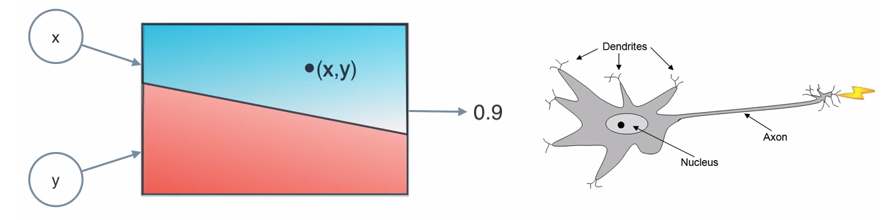
\includegraphics[width=\linewidth,keepaspectratio]{dl9}
\end{center}
{\tiny (Image Credit: A friendly introduction to Deep Learning and Neural Networks -  Luis Serrano)}
\end{frame}



%%%%%%%%%%%%%%%%%%%%%%%%%%%%%%%%%%%%%%%%%%%%%%%%%%%
\begin{frame}[fragile] \frametitle{Composition}
\begin{itemize}
\item If data is not linearly separable, we will need some curve as separator.
\item We can approximate the curve by set of faceted lines. 
\end{itemize}
\begin{center}
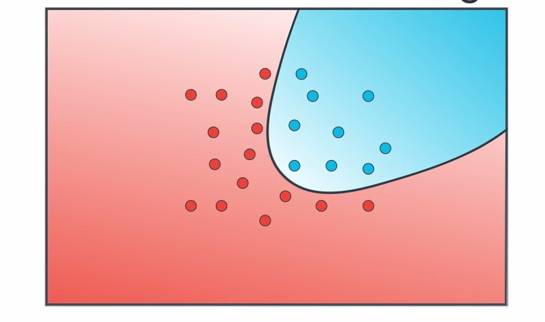
\includegraphics[width=0.7\linewidth,keepaspectratio]{dl10}
\end{center}
{\tiny (Image Credit: A friendly introduction to Deep Learning and Neural Networks -  Luis Serrano)}
\end{frame}

%%%%%%%%%%%%%%%%%%%%%%%%%%%%%%%%%%%%%%%%%%%%%%%%%%%
\begin{frame}[fragile] \frametitle{Composition}
\begin{itemize}
\item Combine two ok solutions.
\item More the facets better the approximation.
\end{itemize}
\begin{center}
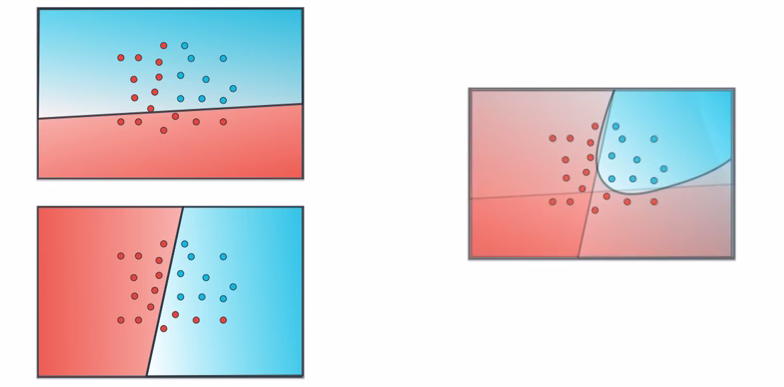
\includegraphics[width=0.8\linewidth,keepaspectratio]{dl11}
\end{center}
{\tiny (Image Credit: A friendly introduction to Deep Learning and Neural Networks -  Luis Serrano)}
\end{frame}

%%%%%%%%%%%%%%%%%%%%%%%%%%%%%%%%%%%%%%%%%%%%%%%%%%%
\begin{frame}[fragile] \frametitle{Composition}
\begin{itemize}
\item If a calculate point comes.
\item We calculate individual probabilities
\item In the network we add them.
\item But we can not have probability more than 1.
\item Put sigmoid to get it mapped to 0 to 1. 0.82 in this case.
\end{itemize}
\begin{center}
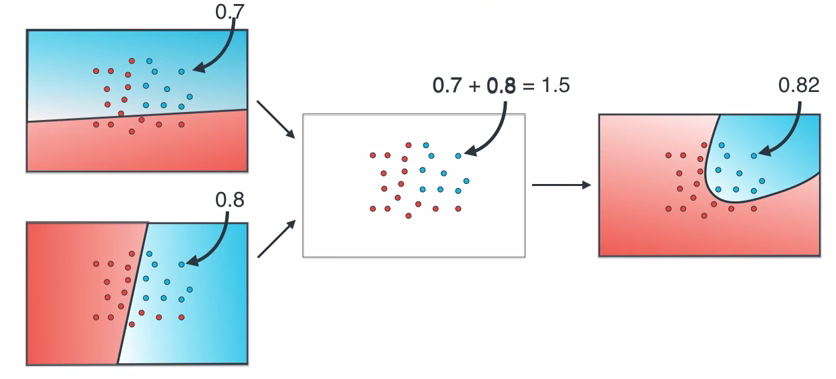
\includegraphics[width=0.7\linewidth,keepaspectratio]{dl12}
\end{center}
{\tiny (Image Credit: A friendly introduction to Deep Learning and Neural Networks -  Luis Serrano)}
\end{frame}

%%%%%%%%%%%%%%%%%%%%%%%%%%%%%%%%%%%%%%%%%%%%%%%%%%%
\begin{frame}[fragile] \frametitle{Weightages}
\begin{itemize}
\item While combining two regions, if you want to have one region with more weight-age.
\item More generalization can be obtained
\item Add bias also
\end{itemize}
\begin{center}
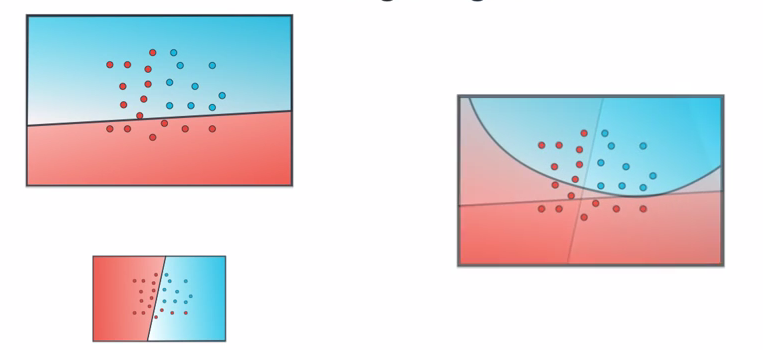
\includegraphics[width=0.8\linewidth,keepaspectratio]{dl13}
\end{center}
{\tiny (Image Credit: A friendly introduction to Deep Learning and Neural Networks -  Luis Serrano)}
\end{frame}

%%%%%%%%%%%%%%%%%%%%%%%%%%%%%%%%%%%%%%%%%%%%%%%%%%%
\begin{frame}[fragile] \frametitle{Result}
\begin{center}
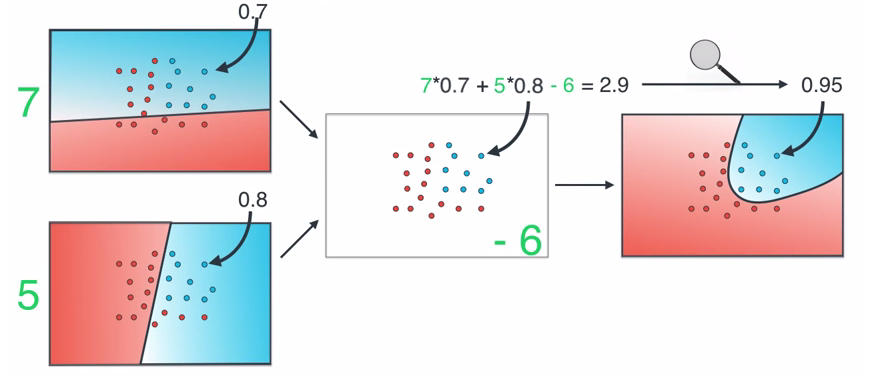
\includegraphics[width=0.8\linewidth,keepaspectratio]{dl14}
\end{center}
{\tiny (Image Credit: A friendly introduction to Deep Learning and Neural Networks -  Luis Serrano)}
\end{frame}

%%%%%%%%%%%%%%%%%%%%%%%%%%%%%%%%%%%%%%%%%%%%%%%%%%%
\begin{frame}[fragile] \frametitle{Network Composition}
\begin{center}
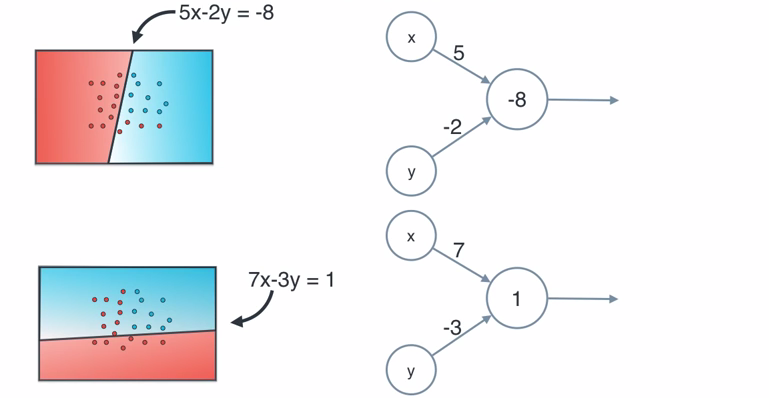
\includegraphics[width=\linewidth,keepaspectratio]{dl15}
\end{center}
{\tiny (Image Credit: A friendly introduction to Deep Learning and Neural Networks -  Luis Serrano)}
\end{frame}


%%%%%%%%%%%%%%%%%%%%%%%%%%%%%%%%%%%%%%%%%%%%%%%%%%%
\begin{frame}[fragile] \frametitle{Neural Network}
\begin{center}
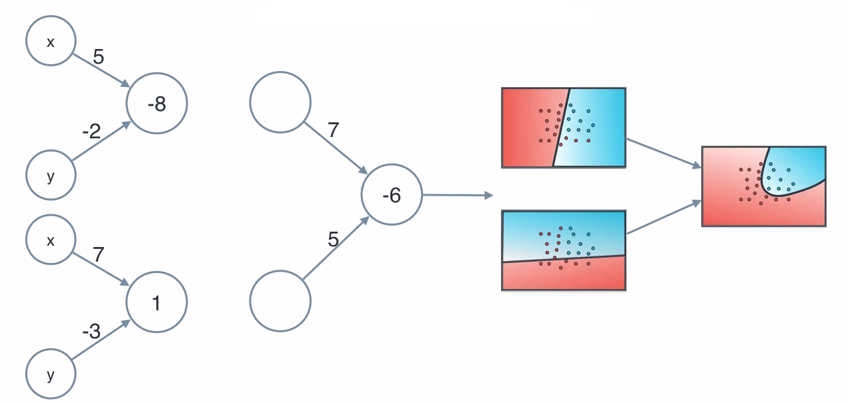
\includegraphics[width=\linewidth,keepaspectratio]{dl16}
\end{center}
Looks like a network, right?

{\tiny (Image Credit: A friendly introduction to Deep Learning and Neural Networks -  Luis Serrano)}
\end{frame}

%%%%%%%%%%%%%%%%%%%%%%%%%%%%%%%%%%%%%%%%%%%%%%%%%%%
\begin{frame}[fragile] \frametitle{Mapping}
Direct Mapping from Deep Learning process to Neural Network architecture
\begin{center}
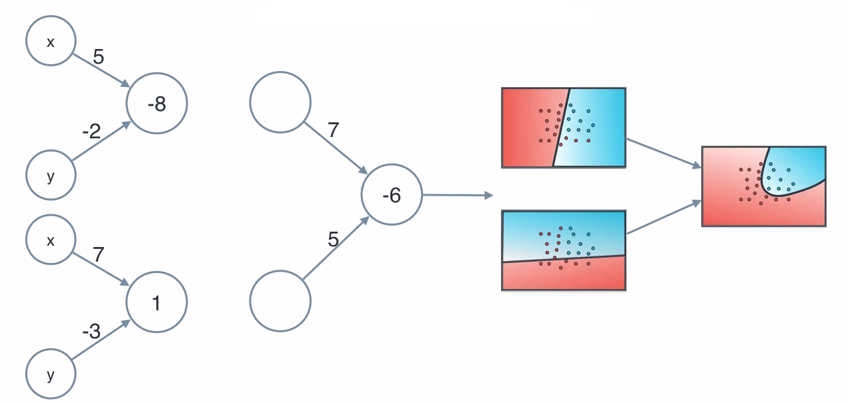
\includegraphics[width=\linewidth,keepaspectratio]{dl16}
\end{center}
{\tiny (Image Credit: A friendly introduction to Deep Learning and Neural Networks -  Luis Serrano)}
\end{frame}


%%%%%%%%%%%%%%%%%%%%%%%%%%%%%%%%%%%%%%%%%%%%%%%%%%%
\begin{frame}[fragile] \frametitle{Architecture}
\begin{center}
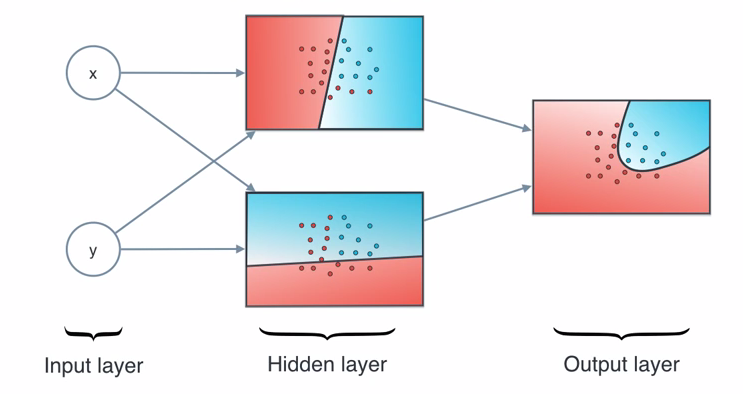
\includegraphics[width=0.8\linewidth,keepaspectratio]{dl18}
\end{center}
\end{frame}

%%%%%%%%%%%%%%%%%%%%%%%%%%%%%%%%%%%%%%%%%%%%%%%%%%%
\begin{frame}[fragile] \frametitle{Neural Network Connections}
3 Nodes in the middle give higher degree output curve
\begin{center}
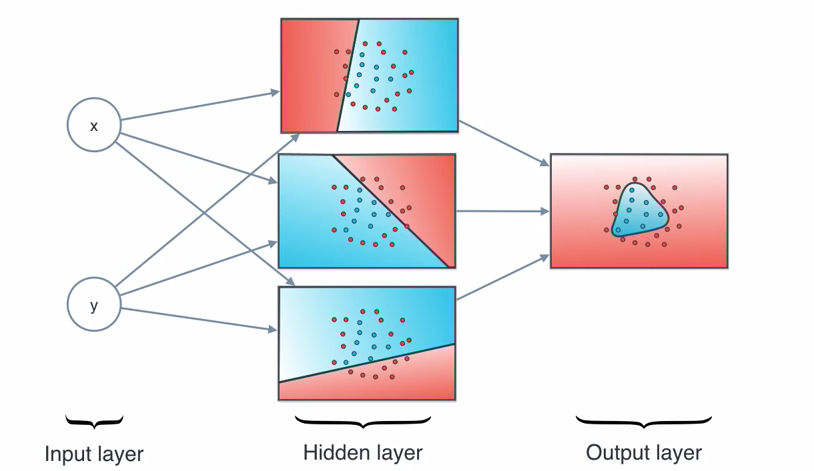
\includegraphics[width=0.8\linewidth,keepaspectratio]{dl19}
\end{center}
\end{frame}

%%%%%%%%%%%%%%%%%%%%%%%%%%%%%%%%%%%%%%%%%%%%%%%%%%%
\begin{frame}[fragile] \frametitle{Partition Formation}
If inputs are 3, then instead of separating lines, we get separating planes.
\begin{center}
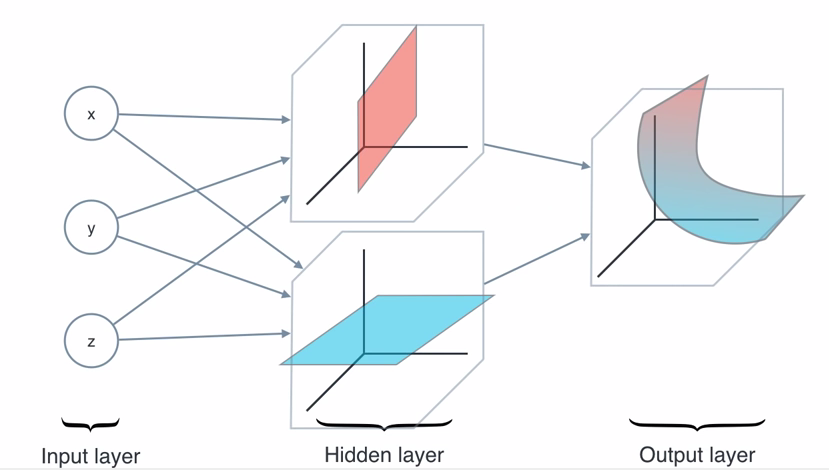
\includegraphics[width=0.8\linewidth,keepaspectratio]{dl20}
\end{center}
\end{frame}


%%%%%%%%%%%%%%%%%%%%%%%%%%%%%%%%%%%%%%%%%%%%%%%%%%%
\begin{frame}[fragile] \frametitle{Deeper Networks}
More hidden layers, more deep, more possibilities of the output separator.
\begin{center}
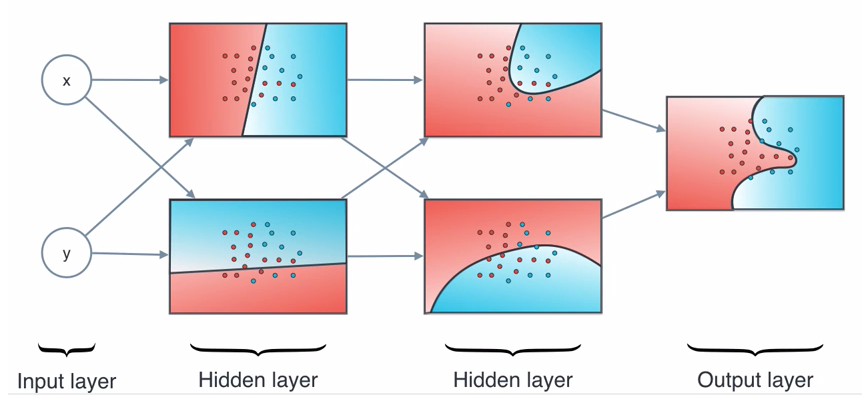
\includegraphics[width=0.8\linewidth,keepaspectratio]{dl21}
\end{center}
\end{frame}


% %%%%%%%%%%%%%%%%%%%%%%%%%%%%%%%%%%%%%%%%%%%%%%%%%%%
% \begin{frame}
  % \begin{center}
    % {\Large Theory: Perceptron}

  % \end{center}
% \end{frame}



% %%%%%%%%%%%%%%%%%%%%%%%%%%%%%%%%%%%%%%%%%%%%%%%%%%%
% \begin{frame}[fragile] \frametitle{Graphical Representation of Perceptron}

% Graphical representation of Perceptron with $3$ binary inputs and a single binary output:
% \begin{center}
% 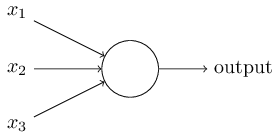
\includegraphics[width=0.6\linewidth,keepaspectratio]{tikz0.png}
% \end{center}


% \end{frame}

% %%%%%%%%%%%%%%%%%%%%%%%%%%%%%%%%%%%%%%%%%%%%%%%%%%%
% \begin{frame}[fragile] \frametitle{Network of Perceptrons}
% \begin{itemize}
% \item A Perceptron takes a number of binary inputs and emits a binary output.
% \item Easy to build a network of such perceptrons, where the
% output from some perceptrons are used in the inputs of other perceptrons:
% \begin{center}
% 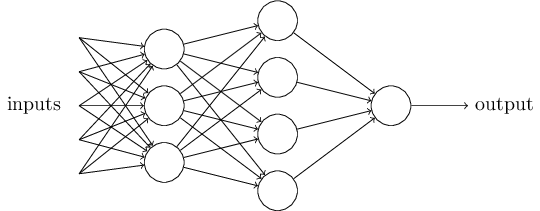
\includegraphics[width=\linewidth,keepaspectratio]{tikz1.png}
% \end{center}
% \end{itemize}
% \end{frame}

% %%%%%%%%%%%%%%%%%%%%%%%%%%%%%%%%%%%%%%%%%%%%%%%%%%%
% \begin{frame}[fragile] \frametitle{Network of Perceptrons}

% The input and outputs are typically represented as their own neurons,
% with the other neurons named {hidden layers}
% \begin{center}
% 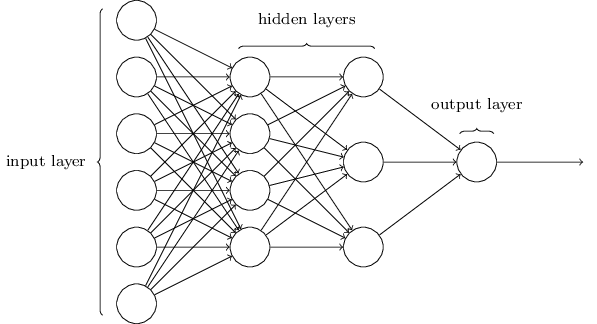
\includegraphics[width=\linewidth,keepaspectratio]{tikz11.png}
% \end{center}

% \end{frame}


% %%%%%%%%%%%%%%%%%%%%%%%%%%%%%%%%%%%%%%%%%%%%%%%%%%%
% \begin{frame}[fragile] \frametitle{Example: The Gates}
% \begin{center}
% 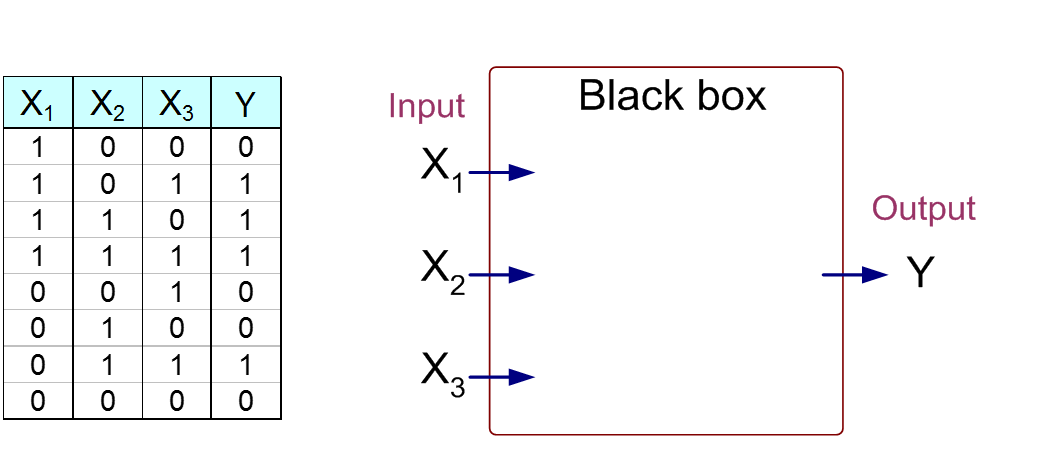
\includegraphics[width=0.8\linewidth,keepaspectratio]{gates1}
% \end{center}

% \begin{itemize}
% \item Output Y is 1 if at least two of the three inputs are equal to 1.
% \item Going to begin with simplest model
% \end{itemize}

% \end{frame}

% %%%%%%%%%%%%%%%%%%%%%%%%%%%%%%%%%%%%%%%%%%%%%%%%%%%
% \begin{frame}[fragile] \frametitle{Using Perceptron}
% \begin{center}
% 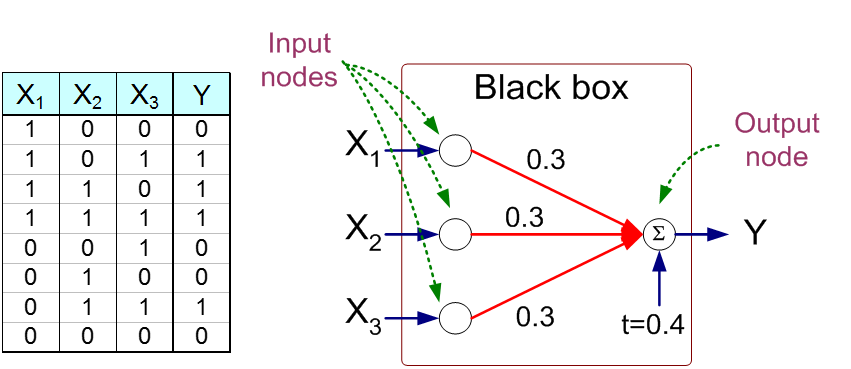
\includegraphics[width=0.8\linewidth,keepaspectratio]{gates2}
% \end{center}

% \begin{itemize}
% \item Perceptron has two types of nodes:
% \begin{itemize}
% \item Input nodes (for the input attributes)
% \item Output node (for the model's output)
% \end{itemize}
% \item Nodes in a neural network are commonly known as neurons.
% \end{itemize}
% \end{frame}


% %%%%%%%%%%%%%%%%%%%%%%%%%%%%%%%%%%%%%%%%%%%%%%%%%%%
% \begin{frame}[fragile] \frametitle{Perceptron}
% \begin{center}
% 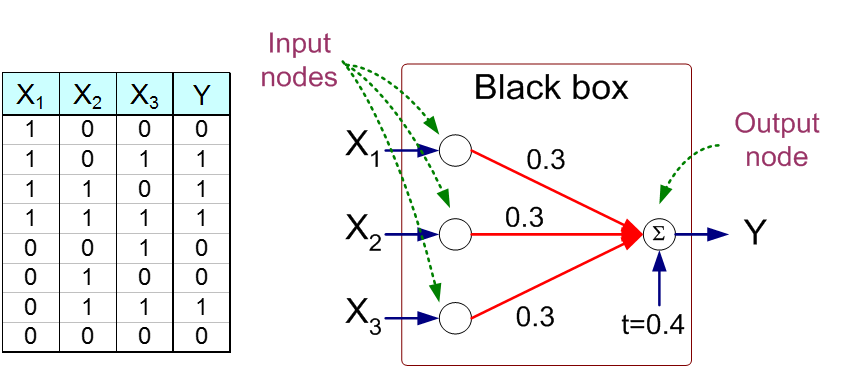
\includegraphics[width=0.6\linewidth,keepaspectratio]{gates3}
% \end{center}

% \begin{itemize}
% \item Each input node is connected to the output node via a weighted link
% \item Weighted link represents the strength of the connection between neurons
% \item Idea: learning the optimal weights
% \end{itemize}
% \end{frame}

% %%%%%%%%%%%%%%%%%%%%%%%%%%%%%%%%%%%%%%%%%%%%%%%%%%%
% \begin{frame}[fragile] \frametitle{Perceptron Output Value}
% \begin{center}
% 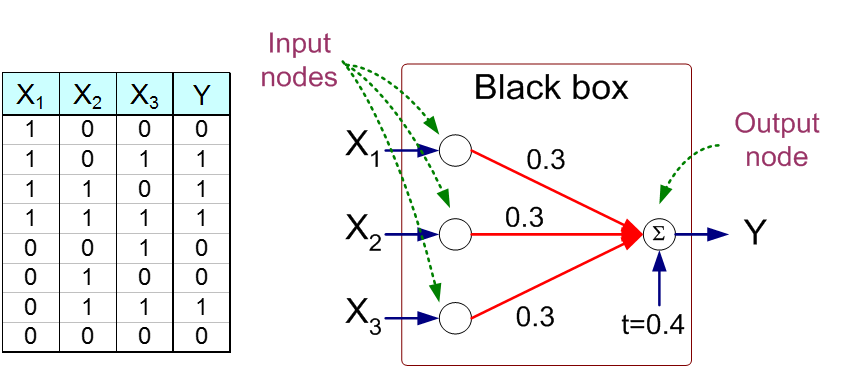
\includegraphics[width=0.6\linewidth,keepaspectratio]{gates4}
% \end{center}

% \begin{itemize}
% \item Weighted sum of inputs, subtracting a bias factor t, and examining sign of the result.
% \item $Y = I(0.3X_1 + 0.3X_2 + 0.3X_3 - 0.4 > 0)$, where $I(z) = {1,0}$ if $z$ is true or false
% \end{itemize}
% \end{frame}

% %%%%%%%%%%%%%%%%%%%%%%%%%%%%%%%%%%%%%%%%%%%%%%%%%%%
% \begin{frame}[fragile] \frametitle{Perceptron General Model}
% \begin{center}
% 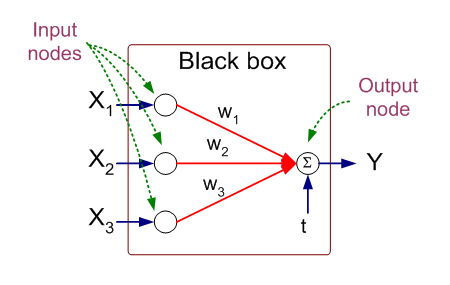
\includegraphics[width=0.6\linewidth,keepaspectratio]{gates5}
% \end{center}

% \begin{itemize}
% \item Model is an assembly of inter-connected nodes and weighted links
% \item Output node sums up each of its input value according to the weights of its links
% \item Compare output node against some threshold $t$

% \item $Y = I(\sum_i w_i X_i - t)$
% \end{itemize}
% \end{frame}

% %%%%%%%%%%%%%%%%%%%%%%%%%%%%%%%%%%%%%%%%%%%%%%%%%%%
% \begin{frame}[fragile] \frametitle{Learning Perceptron Model}
% \begin{center}
% 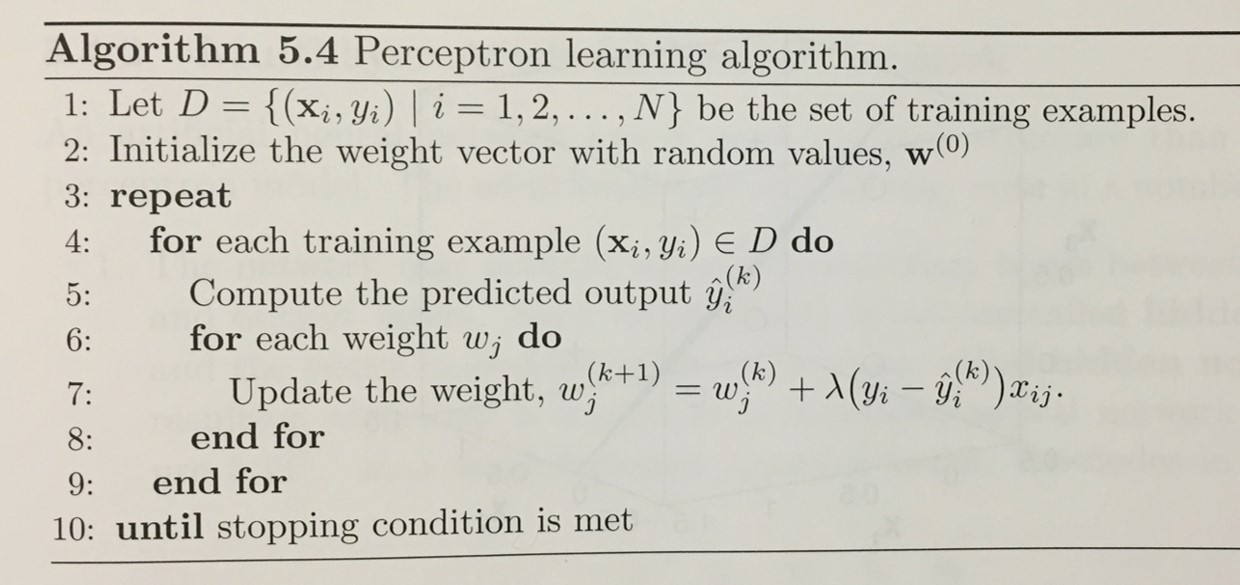
\includegraphics[width=\linewidth,keepaspectratio]{gatesalgo}
% \end{center}
% \end{frame}


% %%%%%%%%%%%%%%%%%%%%%%%%%%%%%%%%%%%%%%%%%%%%%%%%%%%
% \begin{frame}[fragile] \frametitle{Weight Update Formula}
% \begin{center}
% 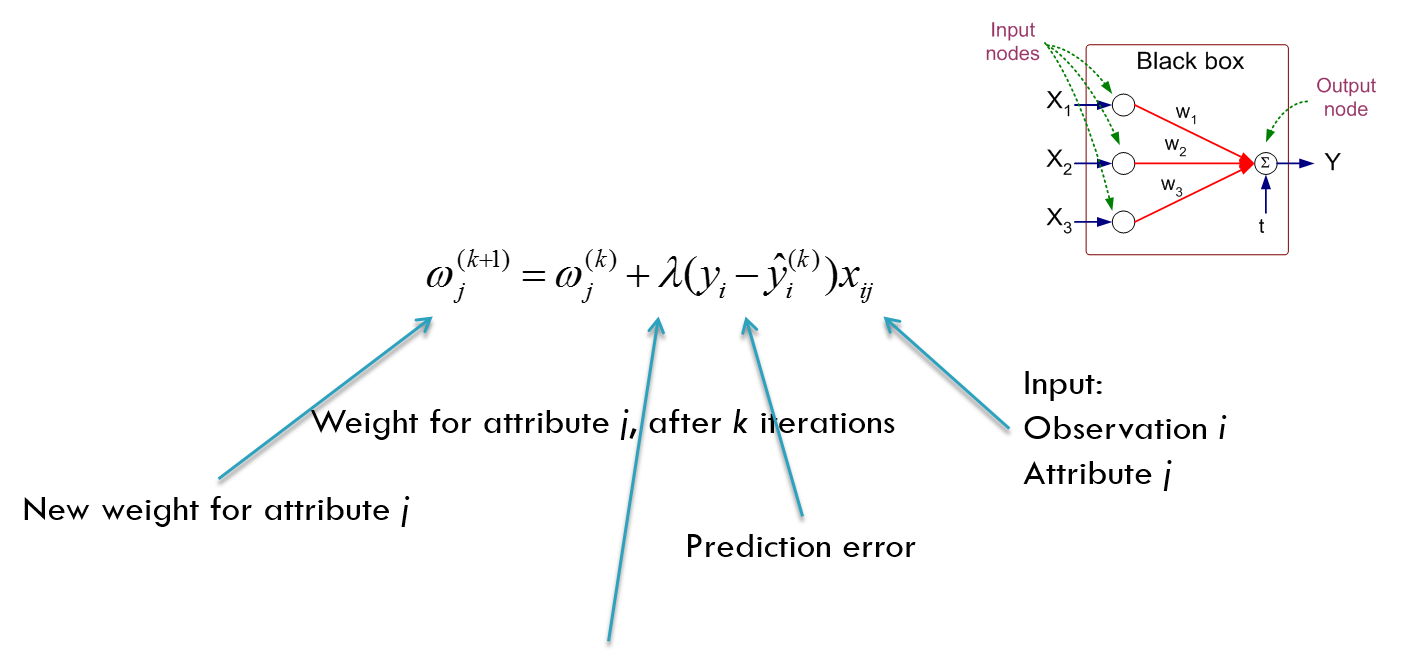
\includegraphics[width=\linewidth,keepaspectratio]{gateswts}
% \end{center}
% \begin{itemize}
% \item Learning rate parameter, between 0 and 1
% \item Closer to 0: SLOW :  new weight mostly influenced by value of old weight
% \item Closer to 1: FAST : more sensitive to error in current iteration
% \end{itemize}
% \end{frame}


%%%%%%%%%%%%%%%%%%%%%%%%%%%%%%%%%%%%%%%%%%%%%%%%%%%%%%%%%%%%%%%%%%%%%%%%%%%%%%%%%%
\begin{frame}[fragile]\frametitle{}
\begin{center}
{\Large Activation Functions}
\end{center}
\end{frame}

%%%%%%%%%%%%%%%%%%%%%%%%%%%%%%%%%%%%%%%%%%%%%%%%%%%
\begin{frame}[fragile] \frametitle{Activation functions }
Non-linearities needed to learn complex (non-linear) representations of data, otherwise the NN would be just a linear function 

\begin{center}
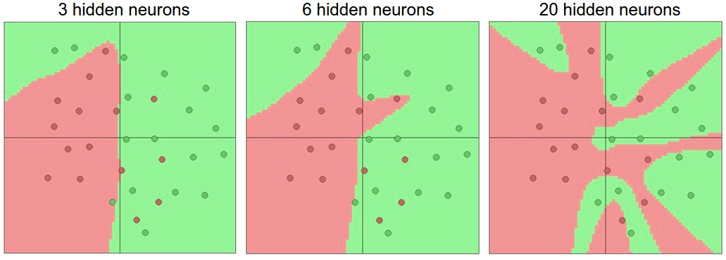
\includegraphics[width=\linewidth,keepaspectratio]{ai57}
\end{center}
More layers and neurons can approximate more complex functions

\tiny{(Reference: Introduction to Deep Learning - Ismini Lourentzou)}
\end{frame}


%%%%%%%%%%%%%%%%%%%%%%%%%%%%%%%%%%%%%%%%%%%%%%%%%%%
\begin{frame}[fragile] \frametitle{Activation functions}

Using a logistic, or sigmoid, activation function has
some benefits in being able to easily take derivatives and the interpret
them using logistic regression.

Other choices have certain benefits that have recently grown in popularity.
Some of these include:
\begin{itemize}
\item hyperbolic tan: $tanh(z) = 2 \sigma(2x) - 1$
\item rectified linear unit: $ReLU(z) = max(0, z)$
\item leaky rectified linear unit
\item maxout
\end{itemize}

\end{frame}


%%%%%%%%%%%%%%%%%%%%%%%%%%%%%%%%%%%%%%%%%%%%%%%%%%%
\begin{frame}[fragile] \frametitle{Activation: Sigmoid}
Takes a real-valued number and ``squashes'' it into range between 0 and 1

\begin{center}
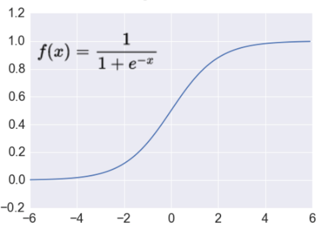
\includegraphics[width=0.4\linewidth,keepaspectratio]{sigmoid}
\end{center}
Sigmoid neurons saturate and kill gradients, thus NN will barely learn


\tiny{(Reference: http://adilmoujahid.com/images/activation.png)}
\end{frame}


%%%%%%%%%%%%%%%%%%%%%%%%%%%%%%%%%%%%%%%%%%%%%%%%%%%
\begin{frame}[fragile] \frametitle{Sigmoid Activation}

\begin{itemize}
\item An important shortcoming of a perceptron is that a small change in
the input values can cause a large change the output because each
node (or neuron) only has two possible states: $0$ or $1$. 
\item A better
solution would be to output a continuum of values, say any number
between $0$ and $1$.
\item Sigmoid function takes any real-valued input and maps it to a real number in the range $(0 1)$ - i.e. between, but not equal to, 0 and 1.
\item The equation for this sigmoid function is:
$\sigma ( x ) = \frac{1}{1 + e^{-x}}$
\end{itemize}
\end{frame}


%%%%%%%%%%%%%%%%%%%%%%%%%%%%%%%%%%%%%%%%%%%%%%%%%%%
\begin{frame}[fragile] \frametitle{Sigmoid Activation}

\begin{itemize}
\item As one option, we could simply have the neuron emit the
value:
\begin{align*}
\sigma(x \cdot w + b) &= \frac{1}{1 + e^{-(x \cdot w + b)}}
\end{align*}
\item For a particularly positive or negative value of $x \cdot w + b$,
the result will be nearly the same as with the perceptron (i.e.,
near $0$ or $1$).
\item For values close to the boundary of the separating
hyperplane, values near $0.5$ will be emitted.
\end{itemize}

\end{frame}

%%%%%%%%%%%%%%%%%%%%%%%%%%%%%%%%%%%%%%%%%%%%%%%%%%%
\begin{frame}[fragile] \frametitle{Logistic Regression}

\begin{itemize}
\item 
This perfectly mimics logistic regression, and in fact uses the
logit function to do so. 
\item In the neural network literature, the
logit function is called the {sigmoid} function, thus leading
to the name {sigmoid neuron} for a neuron that uses it's logic.
\item 
Notice that the previous restriction to binary \textit{inputs} was
not at all needed, and can be easily replaces with continuous input
without an changes needed to the formulas.
\end{itemize}
\end{frame}


%%%%%%%%%%%%%%%%%%%%%%%%%%%%%%%%%%%%%%%%%%%%%%%%%%%
\begin{frame}[fragile] \frametitle{Softmax for Multiclass}
Softmax layer as the output layer

\begin{center}
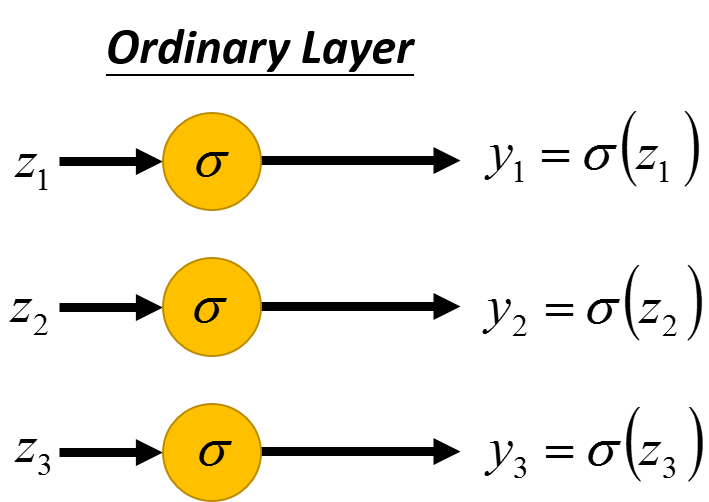
\includegraphics[width=0.6\linewidth,keepaspectratio]{softmax}
\end{center}

\end{frame}

%%%%%%%%%%%%%%%%%%%%%%%%%%%%%%%%%%%%%%%%%%%%%%%%%%%
\begin{frame}[fragile] \frametitle{Softmax Calculations}
Normalization by summation

\begin{center}
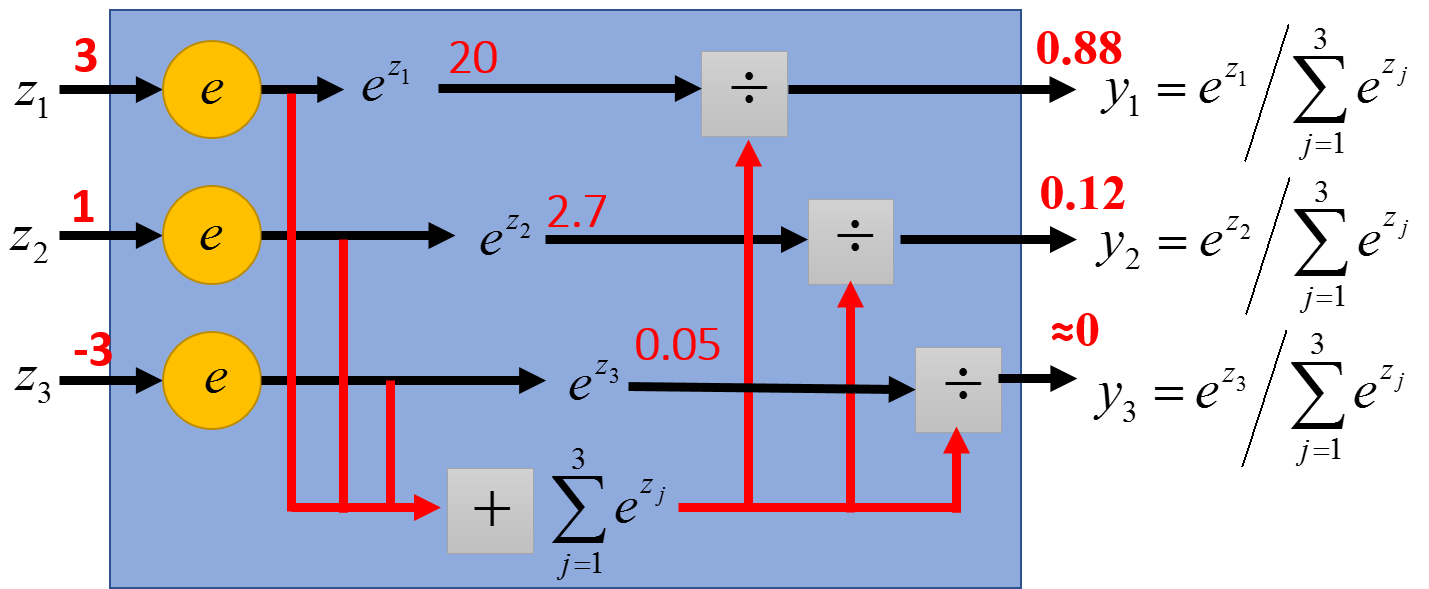
\includegraphics[width=0.8\linewidth,keepaspectratio]{softmaxcalc}
\end{center}

\end{frame}



%%%%%%%%%%%%%%%%%%%%%%%%%%%%%%%%%%%%%%%%%%%%%%%%%%%
\begin{frame}[fragile] \frametitle{Activation: Tanh}
Takes a real-valued number and ``squashes'' it into range between -1 and 1

\begin{center}
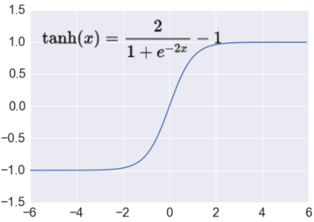
\includegraphics[width=0.4\linewidth,keepaspectratio]{tanh}
\end{center}
Like sigmoid, tanh neurons saturate but unlike sigmoid, output is zero-centered
\tiny{(Reference: http://adilmoujahid.com/images/activation.png)}
\end{frame}


%%%%%%%%%%%%%%%%%%%%%%%%%%%%%%%%%%%%%%%%%%%%%%%%%%%
\begin{frame}[fragile] \frametitle{Activation: Relu}
Takes a real-valued number and thresholds it at zero to its positive value.

\begin{center}
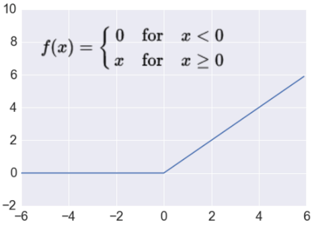
\includegraphics[width=0.4\linewidth,keepaspectratio]{relu1}
\end{center}
\begin{itemize}
\item Trains much faster, 
\item Less expensive operations
\item More expressive 
\item Prevents the gradient vanishing problem
\end{itemize}
\tiny{(Reference: http://adilmoujahid.com/images/activation.png)}
\end{frame}


%%%%%%%%%%%%%%%%%%%%%%%%%%%%%%%%%%%%%%%%%%%%%%%%%%%
\begin{frame}[fragile] \frametitle{Activation: Relu}
\begin{itemize}
\item ReLU units can ``die''
\item Large gradient flowing through a ReLU could cause weights to update in such a way that the neuron will never activate on any datapoint again
gradient flowing through the unit will forever be zero from that point on
\item With a proper setting of the learning rate this is less frequently an issue
\end{itemize}
\tiny{(Reference: Introduction to Deep Learning - Ismini Lourentzou)}
\end{frame}


%%%%%%%%%%%%%%%%%%%%%%%%%%%%%%%%%%%%%%%%%%%%%%%%%%%
\begin{frame}[fragile] \frametitle{Max-out}
\begin{itemize}
\item Activation function in max-out network can be any piecewise linear convex function
\item Learn-able activation function 
\end{itemize}


\begin{center}
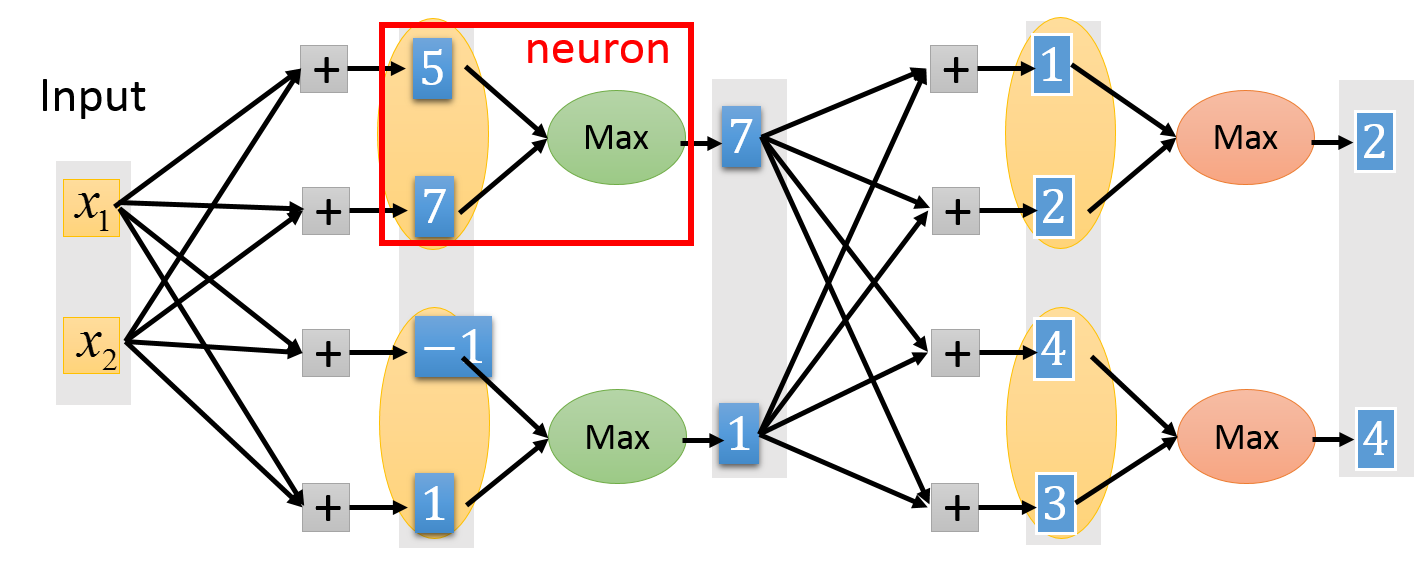
\includegraphics[width=0.8\linewidth,keepaspectratio]{maxout}
\end{center}
\tiny{(Reference:  Deep Learning Tutorial - Hung yi Lee)}
\end{frame}

%%%%%%%%%%%%%%%%%%%%%%%%%%%%%%%%%%%%%%%%%%%%%%%%%%%
\begin{frame}[fragile] \frametitle{ReLU is a special cases of Maxout}
How many pieces depending on how many elements in a group ?

\begin{center}
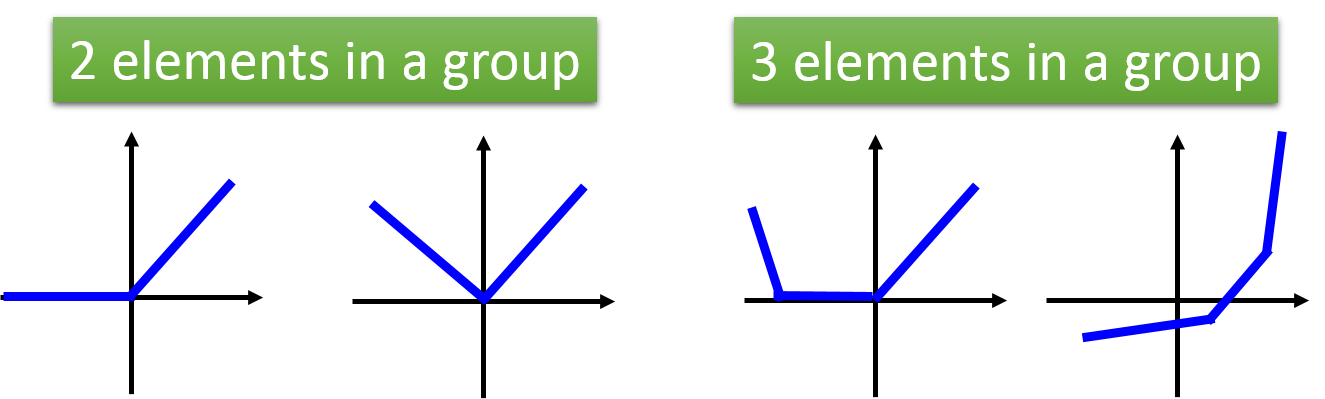
\includegraphics[width=0.8\linewidth,keepaspectratio]{maxoutgroups}
\end{center}
\tiny{(Reference:  Deep Learning Tutorial - Hung yi Lee)}
\end{frame}


%%
%%
%%%%%%%%%%%%%%%%%%%%%%%%%%%%%%%%%%%%%%%%%%%%%%%%%%%%%
%%\begin{frame}[fragile] \frametitle{Elements of Neural Network }
%%
%%\begin{center}
%%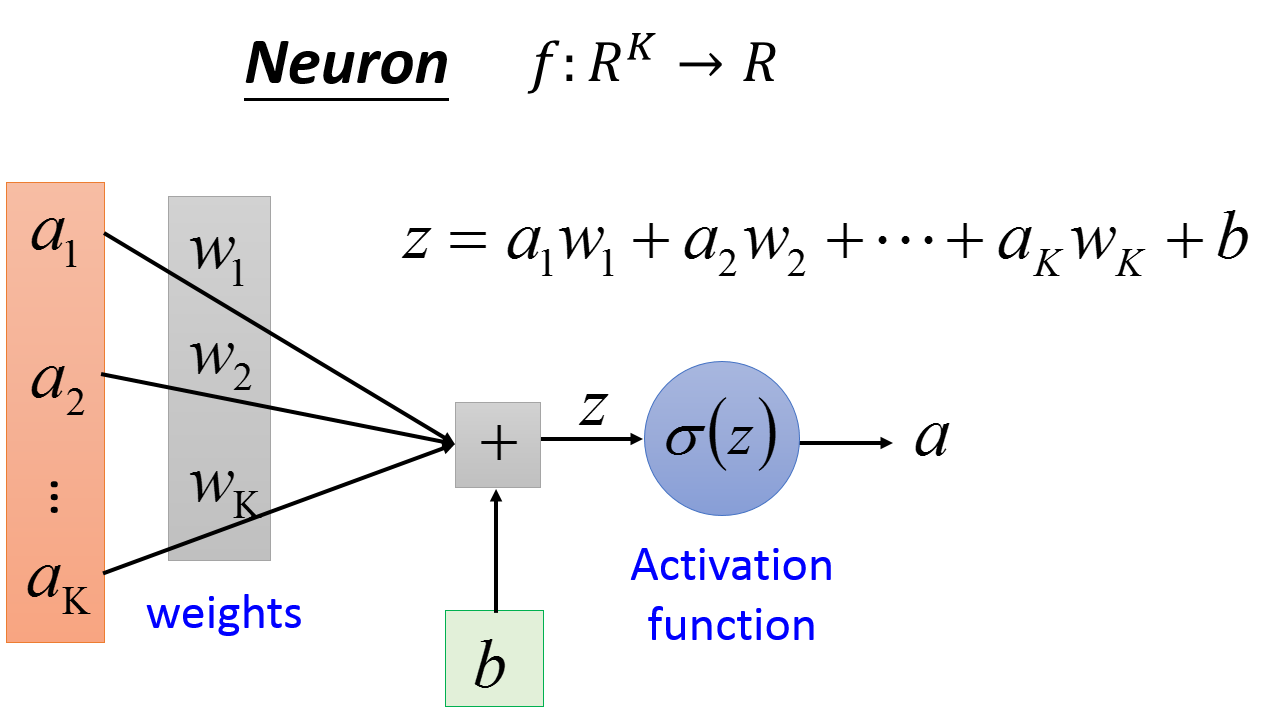
\includegraphics[width=\linewidth,keepaspectratio]{elemnn}
%%\end{center}
%%
%%\end{frame}
%%
%%
%%
%%%%%%%%%%%%%%%%%%%%%%%%%%%%%%%%%%%%%%%%%%%%%%%%%%%%%
%%\begin{frame}[fragile] \frametitle{Deep Neural Network }
%%
%%\begin{center}
%%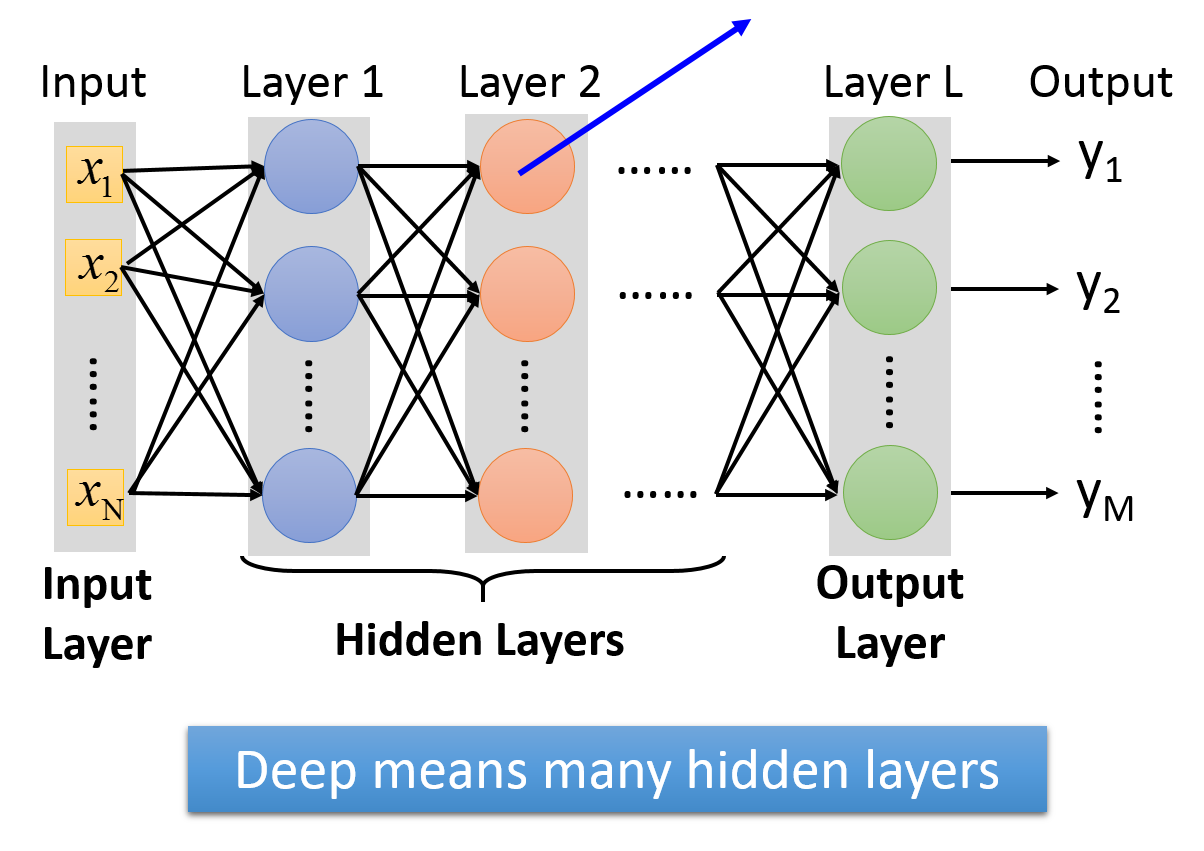
\includegraphics[width=0.8\linewidth,keepaspectratio]{deepnn}
%%\end{center}
%%
%%\end{frame}
%%
%%%%%%%%%%%%%%%%%%%%%%%%%%%%%%%%%%%%%%%%%%%%%%%%%%%%%
%%\begin{frame}[fragile] \frametitle{Example Neural Network }
%%
%%\begin{center}
%%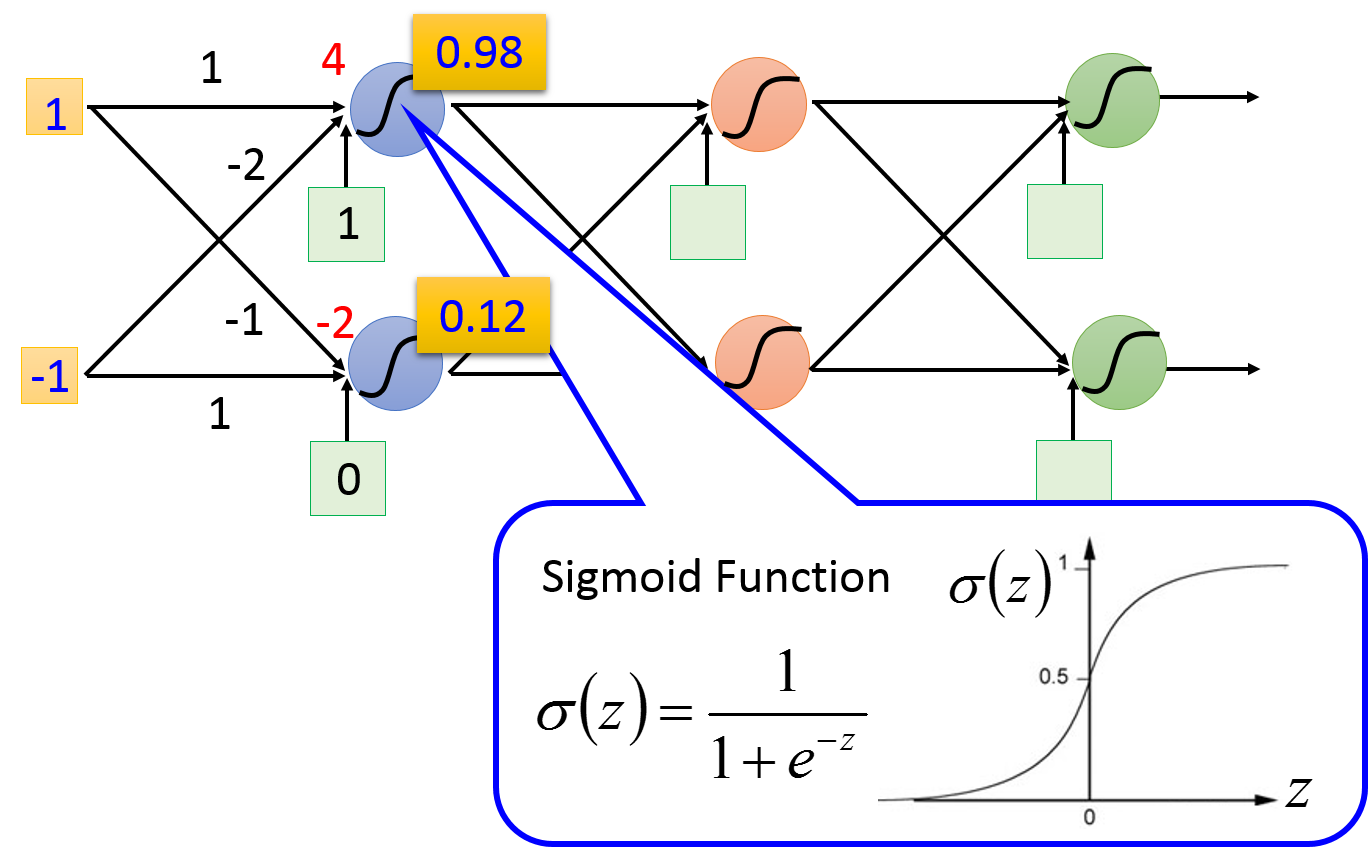
\includegraphics[width=0.8\linewidth,keepaspectratio]{exnn}
%%\end{center}
%%
%%\end{frame}
%%
%%%%%%%%%%%%%%%%%%%%%%%%%%%%%%%%%%%%%%%%%%%%%%%%%%%%%
%%\begin{frame}[fragile] \frametitle{Values in Neural Network }
%%
%%\begin{center}
%%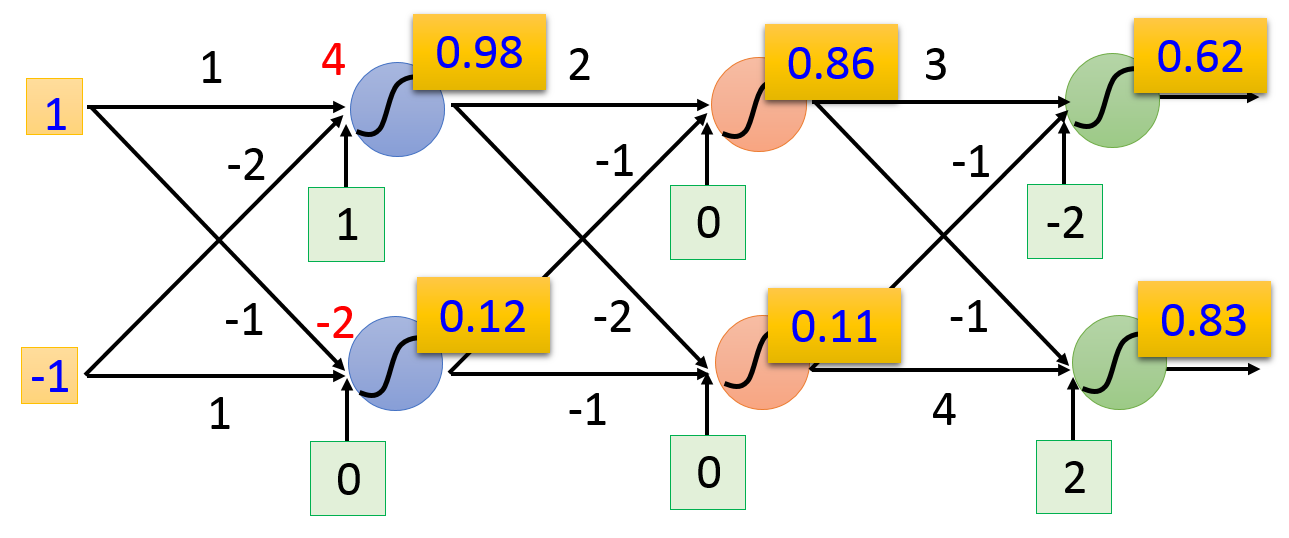
\includegraphics[width=0.8\linewidth,keepaspectratio]{exnnv}
%%\end{center}
%%
%%\end{frame}
%%
%%%%%%%%%%%%%%%%%%%%%%%%%%%%%%%%%%%%%%%%%%%%%%%%%%%%%
%%\begin{frame}[fragile] \frametitle{Parameters in Neural Network }
%%
%%\begin{center}
%%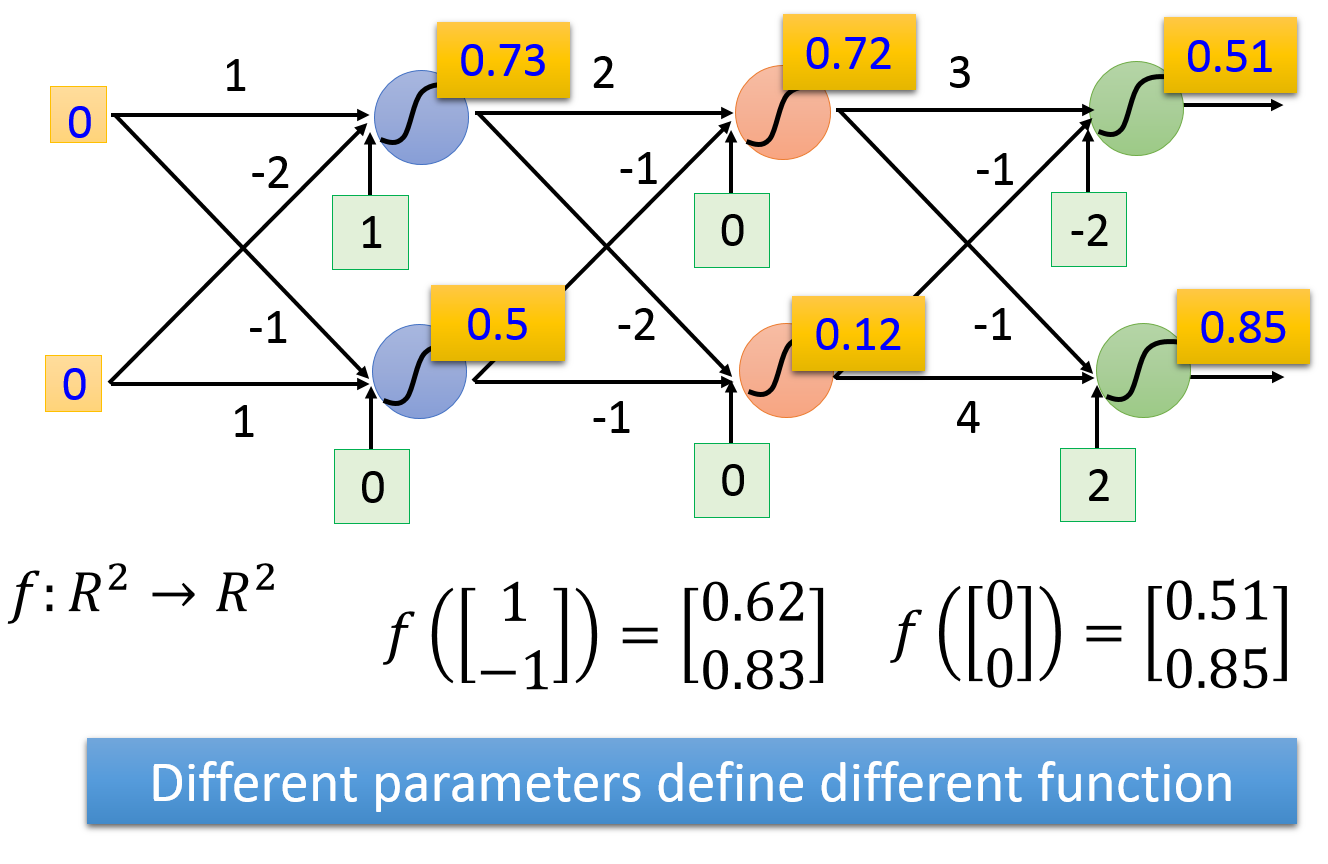
\includegraphics[width=0.8\linewidth,keepaspectratio]{exnnp}
%%\end{center}
%%
%%\end{frame}
%%
%%%%%%%%%%%%%%%%%%%%%%%%%%%%%%%%%%%%%%%%%%%%%%%%%%%%%
%%\begin{frame}[fragile] \frametitle{Matrix Operation}
%%
%%\begin{center}
%%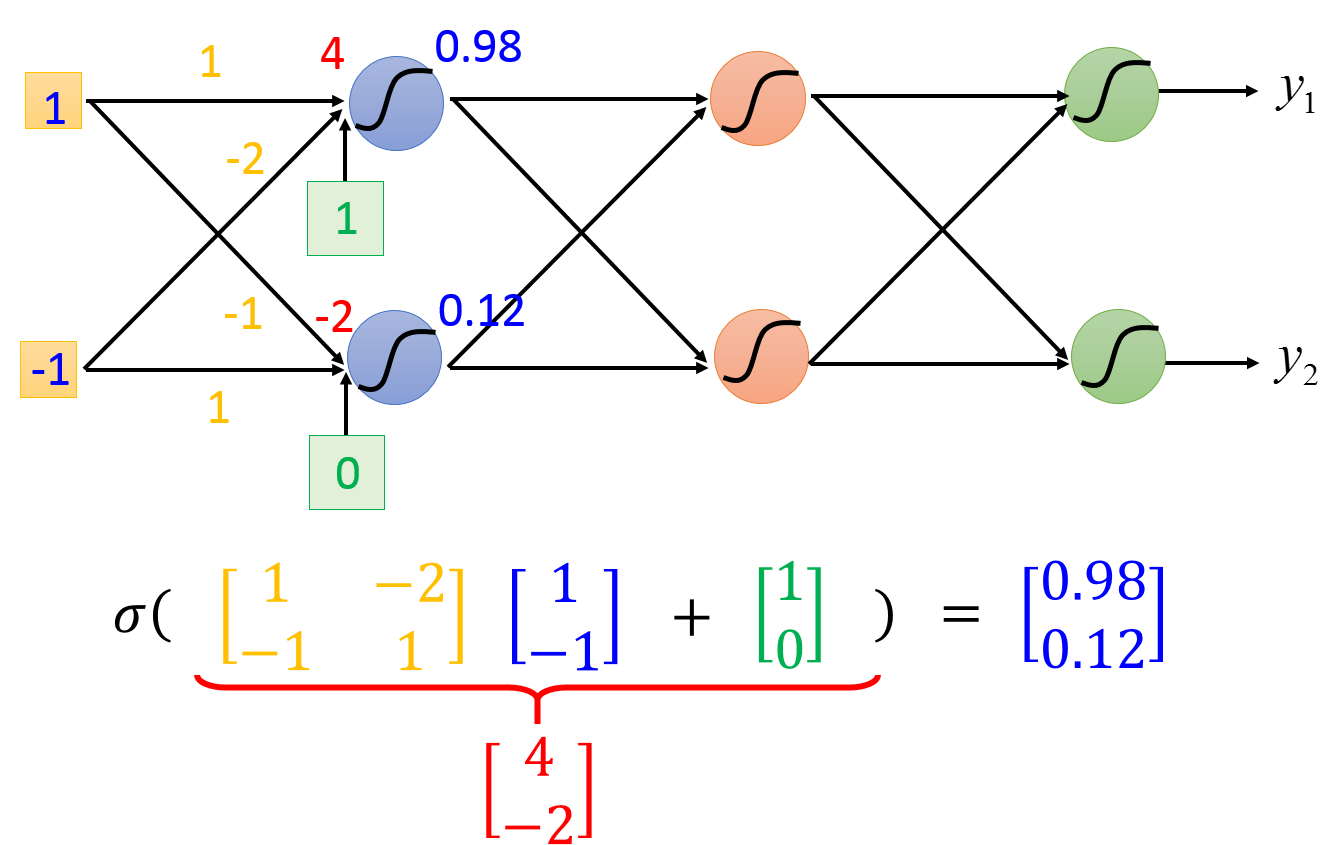
\includegraphics[width=0.8\linewidth,keepaspectratio]{matrixop}
%%\end{center}
%%
%%\end{frame}
%%
%%%%%%%%%%%%%%%%%%%%%%%%%%%%%%%%%%%%%%%%%%%%%%%%%%%%%
%%\begin{frame}[fragile] \frametitle{Layers in Neural Network}
%%
%%\begin{center}
%%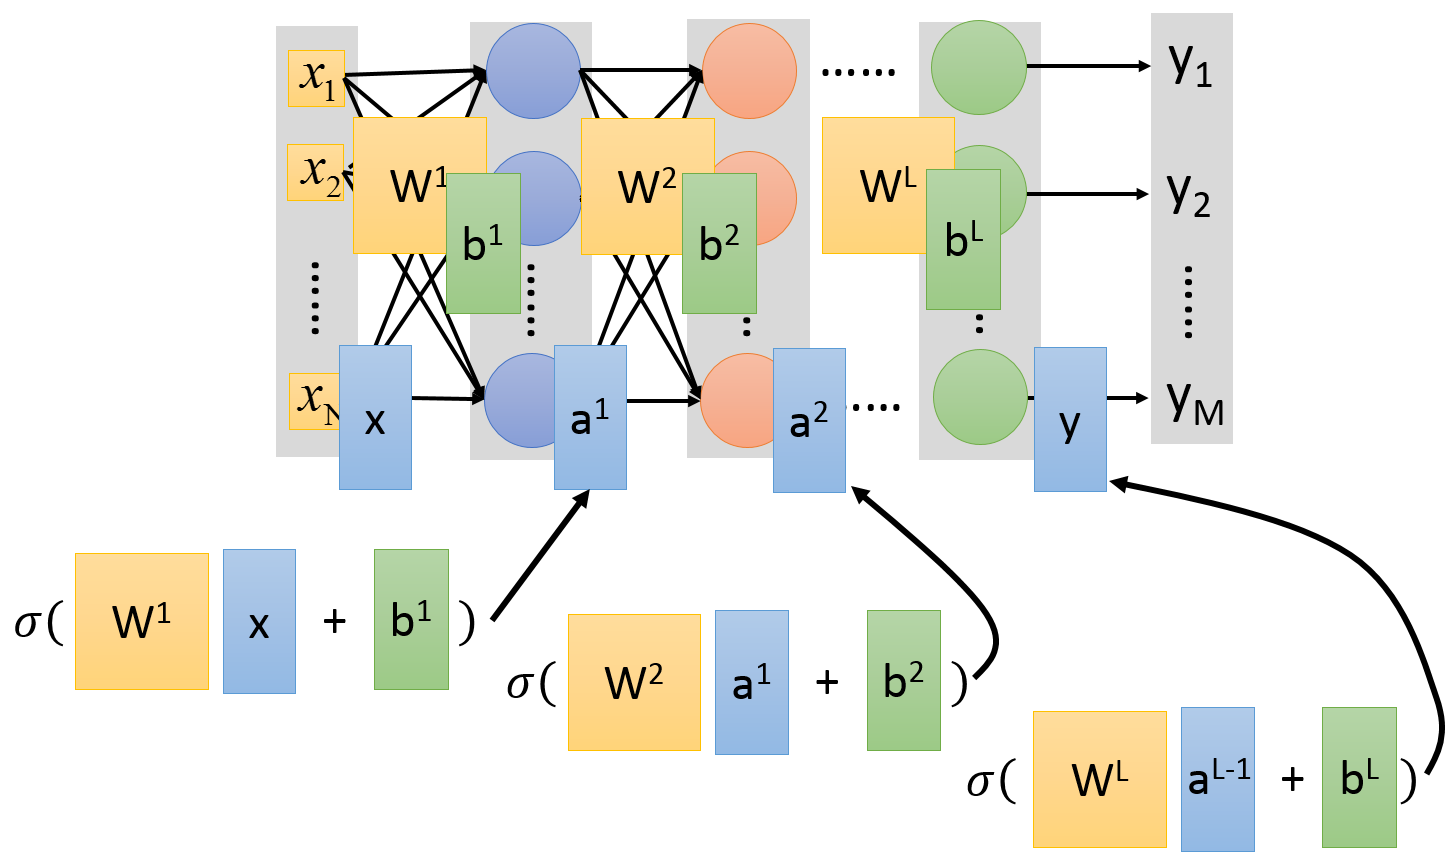
\includegraphics[width=0.8\linewidth,keepaspectratio]{layersnn}
%%\end{center}
%%
%%\end{frame}
%%
%%
%%%%%%%%%%%%%%%%%%%%%%%%%%%%%%%%%%%%%%%%%%%%%%%%%%%%%%
%%%\begin{frame}[fragile] \frametitle{}
%%%
%%%The biological interpretation of a perceptron is this: when it
%%%emits a $1$ this is equivalent to `firing' an electrical pulse,
%%%and when it is $0$ this is when it is not firing. The bias
%%%indicates how difficult it is for this particular node to
%%%send out a signal.
%%%
%%%\end{frame}
%%%
%%%%%%%%%%%%%%%%%%%%%%%%%%%%%%%%%%%%%%%%%%%%%%%%%%%%%%
%%%\begin{frame}[fragile] \frametitle{}
%%%
%%%\begin{center}
%%%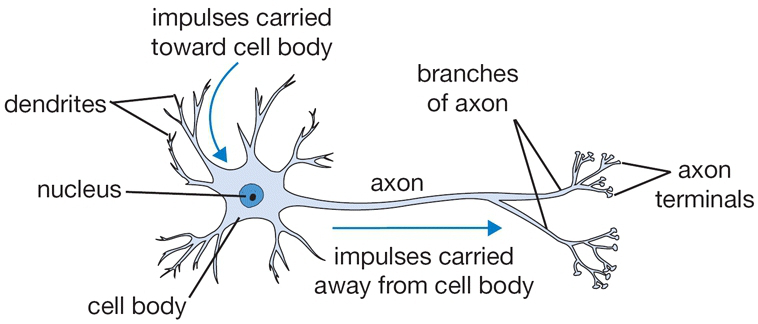
\includegraphics[width=0.4\linewidth]{neuron.png}
%%%\end{center}
%%%
%%%\end{frame}
%%
%%%%%%%%%%%%%%%%%%%%%%%%%%%%%%%%%%%%%%%%%%%%%%%%%%%%%%
%%%\begin{frame}[fragile] \frametitle{}
%%%
%%%\begin{center}
%%%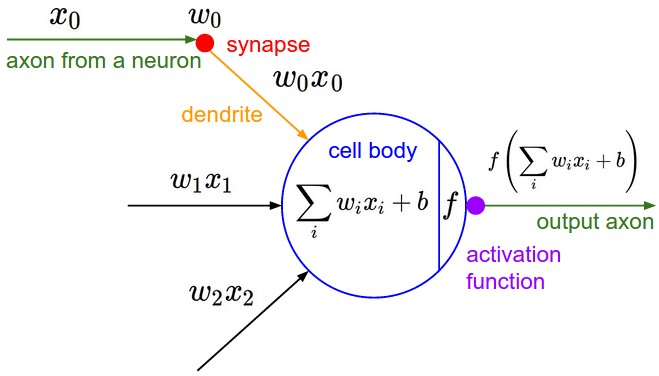
\includegraphics[height=0.7\lineheight]{neuron_model.jpeg}
%%%\end{center}
%%%
%%%\end{frame}
%%
%%
%%%%%%%%%%%%%%%%%%%%%%%%%%%%%%%%%%%%%%%%%%%%%%%%%%%%%%
%%%\begin{frame}[fragile] \frametitle{}
%%%
%%%Notice that the network of nodes I have shown only sends signals
%%%in one direction. This is called a {feed-forward network}.
%%%These are by far the most well-studied types of networks, though
%%%we will (hopefully) have a chance to talk about recurrent neural
%%%networks (RNNs) that allow for loops in the network. The one-directional
%%%nature of feed-forward networks is probably the biggest difference
%%%between artificial neural networks and their biological equivalent.
%%%
%%%\end{frame}
%%
%%%


% %%%%%%%%%%%%%%%%%%%%%%%%%%%%%%%%%%%%%%%%%%%%%%%%%%%
% \begin{frame}[fragile] \frametitle{Rectified Linear Unit (ReLU)}
% \begin{itemize}
% \item Fast to compute
% \item Biological reason (brain research!!)

% \item Vanishing gradient problem

% \end{itemize}

% \begin{center}
% 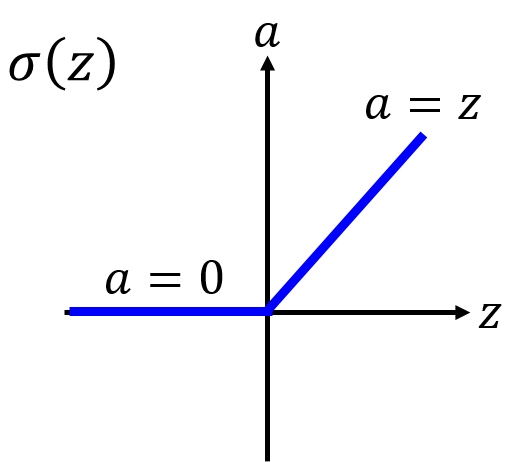
\includegraphics[width=0.6\linewidth,keepaspectratio]{relu}
% \end{center}

% \end{frame}

%%%%%%%%%%%%%%%%%%%%%%%%%%%%%%%%%%%%%%%%%%%%%%%%%%%
\begin{frame}
  \begin{center}
    {\Large Neural Network Formulation}

  \end{center}
\end{frame}

%%%%%%%%%%%%%%%%%%%%%%%%%%%%%%%%%%%%%%%%%%%%%%%%%%%
\begin{frame}[fragile] \frametitle{Feed-forward}
Let’s first consider a 2-layer neural network

\begin{center}
\includegraphics[width=0.4\linewidth,keepaspectratio]{nnff1}
\end{center}

Where,
\begin{itemize}
\item $i$ - the $i^{\text{th}}$ node of the input layer I
\item $j$ - the $j^{\text{th}}$ node of the hidden layer J
\item $k$ - the $k^{\text{th}}$ node of the output layer K
\end{itemize}

The activation function at a node j in the hidden layer takes the value:

\begin{align}
x_{j} &= x_{1} w_{1j} + x_{2} w_{2j} \\[0.5em]
&= \sum_{i \in I} x_{i} w_{i j}
\end{align}

where $x_{i}$ is the value of the $i^{\text{th}}$ input node and $w_{i j}$ is the weight of the connection between $i^{\text{th}}$ input node and the  $j^{\text{th}}$

\tiny{(Ref: A Simple Neural Network - Mathematics - MLNotebook)}
\end{frame}

%%%%%%%%%%%%%%%%%%%%%%%%%%%%%%%%%%%%%%%%%%%%%%%%%%%
\begin{frame}[fragile] \frametitle{Feed-forward}
\begin{itemize}
\item In short: at each hidden layer node, multiply each input value by the connection received by that node and add them together.

\item Note: the weights are initialized when the network is setup. Sometimes they are all set to 1, or often they’re set to some small random value.
\item We apply the activation function on $x_{j}$ at the $j^{\text{th}}$ hidden node and get:

\begin{align}
\mathcal{O}_{j} &= \sigma(x_{j}) \\
&= \sigma(  \xi_{1} w_{1j} + \xi_{2} w_{2j})
\end{align}

\item $\mathcal{O}_{j}$ is the output of the $j^{\text{th}}$ hidden node. 
This is calculated for each of the $j$ nodes in the hidden layer. 
The resulting outputs now become the input for the next layer in the network.
\end{itemize}

\tiny{(Ref: A Simple Neural Network - Mathematics - MLNotebook)}
\end{frame}


%%%%%%%%%%%%%%%%%%%%%%%%%%%%%%%%%%%%%%%%%%%%%%%%%%%
\begin{frame}[fragile] \frametitle{Feed-forward}
\begin{itemize}
\item So for each of the $k$ nodes in $K$:

\begin{align}
\mathcal{O}_{k} &= \sigma(x_{k}) \\
&= \sigma \left( \sum_{j \in J}  \mathcal{O}_{j} w_{jk}  \right)
\end{align}

\item As we’ve reached the end of the network, this is also the end of the feed-foward pass. 
\item So how well did our network do at getting the correct result $\mathcal{O}_{k}$? 
\item As this is the training phase of our network, the true results will be known an we cal calculate the error.
\end{itemize}

\tiny{(Ref: A Simple Neural Network - Mathematics - MLNotebook)}
\end{frame}

%%%%%%%%%%%%%%%%%%%%%%%%%%%%%%%%%%%%%%%%%%%%%%%%%%%
\begin{frame}[fragile] \frametitle{Error}
\begin{itemize}
\item We measure error at the end of each foward pass. 
\item This allows us to quantify how well our network has performed in getting the correct output. 
\item Let’s define $t_k$ as the expected or target value of the $k^{\text{th}}$ node of the output layer $K$. 
\item Then the error $E$ on the entire output is:

$\text{E} = \frac{1}{2} \sum_{k \in K} \left( \mathcal{O}_{k} - t_{k} \right)^{2}$

\item Don't be put off by the random $1/2$ in front there. Its cosmetic. 
Its gets canceled later after derivatives. 
Multiplying by a constant does not affect gradient process. Just its value changes.
\end{itemize}

\tiny{(Ref: A Simple Neural Network - Mathematics - MLNotebook)}
\end{frame}

%%%%%%%%%%%%%%%%%%%%%%%%%%%%%%%%%%%%%%%%%%%%%%%%%%%
\begin{frame}[fragile] \frametitle{Error}
How can we reduce the error?
\begin{itemize}
\item We can’t change the input data, so there are only two other things we can change:
\begin{itemize}
\item the weights going into the activation function
\item the activation function itself
\end{itemize}
\item Lets not look at changing Activation functions, but focus on adjusting weights so that error is minimized.
\item We’re asking, what is the proportion of the error coming from each of the $W_{jk}$ connections 
between the nodes in layer $J$ and the output layer $K$. Or in mathematical terms:
$\frac{\partial{\text{E}}}{\partial{W_{jk}}} =  \frac{\partial{}}{\partial{W_{jk}}}  \frac{1}{2} \sum_{k \in K} \left( \mathcal{O}_{k} - t_{k} \right)^{2}$

\end{itemize}

\tiny{(Ref: A Simple Neural Network - Mathematics - MLNotebook)}
\end{frame}

%%%%%%%%%%%%%%%%%%%%%%%%%%%%%%%%%%%%%%%%%%%%%%%%%%%
\begin{frame}[fragile] \frametitle{Sigmoid Derivatives}

Need derivative of Activation to perform back propagation later on
\begin{align*}
\frac{d}{dx}\sigma ( x ) &= \frac{d}{dx} \left( 1 + e^{ -x }\right)^{-1}\\
&=  -1 \times -e^{-x} \times \left(1 + e^{-x}\right)^{-2}= \frac{ e^{-x} }{ \left(1 + e^{-x}\right)^{2} } \\
&= \frac{\left(1 + e^{-x}\right) - 1}{\left(1 + e^{-x}\right)^{2}} \\
&= \frac{\left(1 + e^{-x}\right) }{\left(1 + e^{-x}\right)^{2}} - \frac{1}{\left(1 + e^{-x}\right)^{2}} \\
&= \frac{1}{\left(1 + e^{-x}\right)} - \left( \frac{1}{\left(1 + e^{-x}\right)} \right)^{2} \\[0.5em]
&= \sigma ( x ) - \sigma ( x ) ^ {2}
\end{align*}

Note:  plus minus 1 on numerator, in the middle step.

\end{frame}

%%%%%%%%%%%%%%%%%%%%%%%%%%%%%%%%%%%%%%%%%%%%%%%%%%%
\begin{frame}[fragile] \frametitle{Sigmoid Derivatives}

Therefore, we can write the derivative of the sigmoid function as:

$\sigma^{\prime}( x ) = \sigma (x ) \left( 1 - \sigma ( x ) \right)$

The sigmoid function has the nice property that its derivative is very simple: a bonus when we want to hard-code this into our NN later on.
\end{frame}




%%%%%%%%%%%%%%%%%%%%%%%%%%%%%%%%%%%%%%%%%%%%%%%%%%%
\begin{frame}[fragile] \frametitle{Back-propagation Derivation}

\begin{itemize}
\item Note:  the derivative of the sum is equal to the sum of the derivatives i.e. we can move the derivative term inside of the summation:

$\frac{\partial{\text{E}}}{\partial{W_{jk}}} =  \frac{1}{2} \sum_{k \in K} \frac{\partial{}}{\partial{W_{jk}}} \left( \mathcal{O}_{k} - t_{k} \right)^{2}$

\item The weight $W_{1k}$ does not affect connection $W_{1k}$ therefore the change in $W_{jk}$ with respect to any node other than the current $k$ is zero. Thus the summation goes away:

$\frac{\partial{\text{E}}}{\partial{W_{jk}}} =  \frac{1}{2} \frac{\partial{}}{\partial{W_{jk}}}  \left( \mathcal{O}_{k} - t_{k} \right)^{2}$

\item Apply the power rule knowing that $t_k$ is a constant:

\begin{align}
\frac{\partial{\text{E}}}{\partial{W_{jk}}} &=  \frac{1}{2} \times 2 \times \left( \mathcal{O}_{k} - t_{k} \right) \frac{\partial{}}{\partial{W_{jk}}}  \left( \mathcal{O}_{k}\right) \\
 &=  \left( \mathcal{O}_{k} - t_{k} \right) \frac{\partial{}}{\partial{W_{jk}}}  \left( \mathcal{O}_{k}\right)
\end{align}

\end{itemize}

\tiny{(Ref: A Simple Neural Network - Mathematics - MLNotebook)}
\end{frame}


%%%%%%%%%%%%%%%%%%%%%%%%%%%%%%%%%%%%%%%%%%%%%%%%%%%
\begin{frame}[fragile] \frametitle{Back-propagation Derivation}

\begin{itemize}
\item The leftover derivative is the chage in the output values with respect to the weights. 
\item Substituting $\mathcal{O}_{k} = \sigma(x_{k})$ and the sigmoid derivative
$\sigma^{\prime}( x ) = \sigma (x ) \left( 1 - \sigma ( x ) \right)$:

$\frac{\partial{\text{E}}}{\partial{W_{jk}}} =  \left( \mathcal{O}_{k} - t_{k} \right) \sigma (x ) \left( 1 - \sigma ( x ) \right) \frac{\partial{}}{\partial{W_{jk}}}  \left( x_{k}\right)$

\item the final derivative, the input value $x_{k}$ is just $\mathcal{O}_{j} W_{jk}$ i.e. output of the previous layer times the weight to this layer. 

\item So the change in $\mathcal{O}_{j} w_{jk}$ with respect to $w_{jk}$ just gives us the 
output value of the previous layer $\mathcal{O}_{j}$ and so the full derivative becomes:

\begin{align}
\frac{\partial{\text{E}}}{\partial{W_{jk}}}  &=  \left( \mathcal{O}_{k} - t_{k} \right) \sigma (x ) \left( 1 - \sigma ( x ) \right) \frac{\partial{}}{\partial{W_{jk}}}  \left( \mathcal{O}_{j} W_{jk} \right) \\[0.5em]
&=\left( \mathcal{O}_{k} - t_{k} \right) \sigma (x )  \left( 1 - \mathcal{O}_{k}  \right) \mathcal{O}_{j} 
\end{align}

\item We can replace the sigmoid function with the output of the layer
\end{itemize}

\tiny{(Ref: A Simple Neural Network - Mathematics - MLNotebook)}
\end{frame}

%%%%%%%%%%%%%%%%%%%%%%%%%%%%%%%%%%%%%%%%%%%%%%%%%%%
\begin{frame}[fragile] \frametitle{Back-propagation Derivation}

\begin{itemize}
\item The derivative of the error function with respect to the weights is then: 

$\frac{\partial{\text{E}}}{\partial{W_{jk}}}  =\left( \mathcal{O}_{k} - t_{k} \right) \mathcal{O}_{k}  \left( 1 - \mathcal{O}_{k}  \right) \mathcal{O}_{j}$

\item We group the terms involving $k$ and define: $\delta_{k} = \mathcal{O}_{k}  \left( 1 - \mathcal{O}_{k}  \right)  \left( \mathcal{O}_{k} - t_{k} \right)$

\item And therefore: $\frac{\partial{\text{E}}}{\partial{W_{jk}}}  = \mathcal{O}_{j} \delta_{k}$

\item So we have an expression for the amount of error, called ‘delta' ($\delta_{k}$), 
on the weights from the nodes in $J$ to each node $k$ in $K$. 
\item But how does this help us to improve out network?
\item We need to back propagate the error.
\end{itemize}

\tiny{(Ref: A Simple Neural Network - Mathematics - MLNotebook)}
\end{frame}

%%%%%%%%%%%%%%%%%%%%%%%%%%%%%%%%%%%%%%%%%%%%%%%%%%%
\begin{frame}[fragile] \frametitle{Back-propagation - Gradients}

\begin{itemize}
\item Back propagation takes the error function we found in the previous section, uses it to calculate the error on the current layer and updates the weights to that layer by some amount.
\item So far we’ve only looked at the error on the output layer, what about the hidden layer? 
\item This also has an error, but the error here depends on the output layer’s error too (because this is where the difference between the target $t_k$ and output $\mathcal{O}_{k}$ can be calculated). 
\item Lets have a look at the error on the weights of the hidden layer $W_{ij}$:

$\frac{\partial{\text{E}}}{\partial{W_{ij}}} =  \frac{\partial{}}{\partial{W_{ij}}}  \frac{1}{2} \sum_{k \in K} \left( \mathcal{O}_{k} - t_{k} \right)^{2}$

\end{itemize}

\tiny{(Ref: A Simple Neural Network - Mathematics - MLNotebook)}
\end{frame}

%%%%%%%%%%%%%%%%%%%%%%%%%%%%%%%%%%%%%%%%%%%%%%%%%%%
\begin{frame}[fragile] \frametitle{Back-propagation - Gradients}

\begin{itemize}
\item Now, unlike before, we cannot just drop the summation as the derivative is not directly acting on a subscript $k$ in the 
summation. 
\item We should be careful to note that the output from every node in $J$ is actually connected to each of the nodes in $K$ 
so the summation should stay. 
\item But we can still use the same tricks as before: 
lets use the power rule again and move the derivative inside (because the summation is finite):

\begin{align}
\frac{\partial{\text{E}}}{\partial{W_{ij}}} &=  \frac{1}{2} \times 2 \times  \frac{\partial{}}{\partial{W_{ij}}}   \sum_{k \in K} \left( \mathcal{O}_{k} - t_{k} \right)  \mathcal{O}_{k} \\
&= \sum_{k \in K} \left( \mathcal{O}_{k} - t_{k} \right) \frac{\partial{}}{\partial{W_{ij}}} \mathcal{O}_{k}
 \end{align}
 
\end{itemize}

\tiny{(Ref: A Simple Neural Network - Mathematics - MLNotebook)}
\end{frame}

%%%%%%%%%%%%%%%%%%%%%%%%%%%%%%%%%%%%%%%%%%%%%%%%%%%
\begin{frame}[fragile] \frametitle{Back-propagation - Gradients}

\begin{itemize}
\item Again, we substitute $\mathcal{O}_{k} = \sigma( x_{k})$ and its derivative and revert back to our output notation:

\begin{align}
\frac{\partial{\text{E}}}{\partial{W_{ij}}} &= \sum_{k \in K} \left( \mathcal{O}_{k} - t_{k} \right) \frac{\partial{}}{\partial{W_{ij}}} (\sigma(x_{k}) )\\
&= \sum_{k \in K} \left( \mathcal{O}_{k} - t_{k} \right) \sigma(x_{k}) \left( 1 - \sigma(x_{k}) \right) \frac{\partial{}}{\partial{W_{ij}}} (x_{k}) \\
&= \sum_{k \in K} \left( \mathcal{O}_{k} - t_{k} \right) \mathcal{O}_{k} \left( 1 - \mathcal{O}_{k} \right) \frac{\partial{}}{\partial{W_{ij}}} (x_{k})
 \end{align}
 
\item Let’s use the chain rule to break apart this derivative in terms of the output from $J$:

$\frac{\partial{ x_{k}}}{\partial{W_{ij}}} = \frac{\partial{ x_{k}}}{\partial{\mathcal{O}_{j}}}\frac{\partial{\mathcal{O}_{j}}}{\partial{W_{ij}}}$

\end{itemize}

\tiny{(Ref: A Simple Neural Network - Mathematics - MLNotebook)}
\end{frame}


%%%%%%%%%%%%%%%%%%%%%%%%%%%%%%%%%%%%%%%%%%%%%%%%%%%
\begin{frame}[fragile] \frametitle{Back-propagation - Gradients}

\begin{itemize}
\item The change of the input to the $k^{\text{th}}$ node with respect to the output from the $j^{\text{th}}$ 
node is down to a product with the weights, therefore this derivative just becomes the weights $W_{jk}$. 
\item The final derivative has nothing to do with the subscript $k$ anymore, 
\item so we’re free to move this around - lets put it at the beginning:

\begin{align}
\frac{\partial{\text{E}}}{\partial{W_{ij}}} &= \frac{\partial{\mathcal{O}_{j}}}{\partial{W_{ij}}}  \sum_{k \in K} \left( \mathcal{O}_{k} - t_{k} \right) \mathcal{O}_{k} \left( 1 - \mathcal{O}_{k} \right) W_{jk}
 \end{align}

\end{itemize}

\tiny{(Ref: A Simple Neural Network - Mathematics - MLNotebook)}
\end{frame}

%%%%%%%%%%%%%%%%%%%%%%%%%%%%%%%%%%%%%%%%%%%%%%%%%%%
\begin{frame}[fragile] \frametitle{Back-propagation - Gradients}

Remembering that the output of the node $j$ is just $\mathcal{O}_{j} = \sigma(x_{j})$ and we know the derivative of this function too:

\begin{align}
\frac{\partial{\text{E}}}{\partial{W_{ij}}} &= \frac{\partial{}}{\partial{W_{ij}}}\sigma(x_{j})  \sum_{k \in K} \left( \mathcal{O}_{k} - t_{k} \right) \mathcal{O}_{k} \left( 1 - \mathcal{O}_{k} \right) W_{jk} \\
&= \sigma(x_{j}) \left( 1 - \sigma(x_{j}) \right)  \frac{\partial{x_{j} }}{\partial{W_{ij}}} \sum_{k \in K} \left( \mathcal{O}_{k} - t_{k} \right) \mathcal{O}_{k} \left( 1 - \mathcal{O}_{k} \right) W_{jk} \\
&= \mathcal{O}_{j} \left( 1 - \mathcal{O}_{j} \right)  \frac{\partial{x_{j} }}{\partial{W_{ij}}} \sum_{k \in K} \left( \mathcal{O}_{k} - t_{k} \right) \mathcal{O}_{k} \left( 1 - \mathcal{O}_{k} \right) W_{jk}
 \end{align}
 

\tiny{(Ref: A Simple Neural Network - Mathematics - MLNotebook)}
\end{frame}

%%%%%%%%%%%%%%%%%%%%%%%%%%%%%%%%%%%%%%%%%%%%%%%%%%%
\begin{frame}[fragile] \frametitle{Back-propagation - Gradients}

\begin{itemize}
\item The final derivative is straightforward too, the derivative of the input to j with respect to the weights is just the previous input, 
which in our case is $\mathcal{O}_{i}$,

\begin{align}
\frac{\partial{\text{E}}}{\partial{W_{ij}}} &= \mathcal{O}_{j} \left( 1 - \mathcal{O}_{j} \right)  \mathcal{O}_{i} \sum_{k \in K} \left( \mathcal{O}_{k} - t_{k} \right) \mathcal{O}_{k} \left( 1 - \mathcal{O}_{k} \right) W_{jk}
 \end{align}
 
\item Almost there! Recall that we defined $\delta_{k}$ earlier, lets sub that in:
 
\begin{align}
\frac{\partial{\text{E}}}{\partial{W_{ij}}} &= \mathcal{O}_{j} \left( 1 - \mathcal{O}_{j} \right)  \mathcal{O}_{i} \sum_{k \in K} \delta_{k} W_{jk}
 \end{align}
 
 
\end{itemize}

\tiny{(Ref: A Simple Neural Network - Mathematics - MLNotebook)}
\end{frame}


%%%%%%%%%%%%%%%%%%%%%%%%%%%%%%%%%%%%%%%%%%%%%%%%%%%
\begin{frame}[fragile] \frametitle{Back-propagation - Gradients}

\begin{itemize}
\item To clean this up, we now define the ‘delta’ for our hidden layer:

$\delta_{j} = \mathcal{O}_{i} \left( 1 - \mathcal{O}_{j} \right)   \sum_{k \in K} \delta_{k} W_{jk}$


\item Thus, the amount of error on each of the weights going into our hidden layer:

$\frac{\partial{\text{E}}}{\partial{W_{ij}}}  = \mathcal{O}_{i} \delta_{j}$

\item Note: the reason for the name back propagation is that we must calculate the errors at the far end of the network and work backwards to be able to calculate the weights at the front.


\end{itemize}

\tiny{(Ref: A Simple Neural Network - Mathematics - MLNotebook)}
\end{frame}


%%%%%%%%%%%%%%%%%%%%%%%%%%%%%%%%%%%%%%%%%%%%%%%%%%%
\begin{frame}[fragile] \frametitle{Back-propagation - Algorithm}

\begin{itemize}
\item Input the data into the network and feed-forward
\item For each of the output nodes calculate: $\delta_{k} = \mathcal{O}_{k}  \left( 1 - \mathcal{O}_{k}  \right)  \left( \mathcal{O}_{k} - t_{k} \right)$
\item For each of the hidden layer nodes calculate: $\delta_{j} = \mathcal{O}_{i} \left( 1 - \mathcal{O}_{j} \right)   \sum_{k \in K} \delta_{k} W_{jk}$
\item Calculate the changes that need to be made to the weights and bias terms:
\begin{align}
\Delta W &= -\eta \ \delta_{l} \ \mathcal{O}_{l-1} \\
\Delta\theta &= -\eta \ \delta_{l}
\end{align}
\item Update the weights and biases across the network:
\begin{align}
W + \Delta W &\rightarrow W \\
\theta + \Delta\theta &\rightarrow \theta
\end{align}
\end{itemize}

\tiny{(Ref: A Simple Neural Network - Mathematics - MLNotebook)}
\end{frame}


%%%%%%%%%%%%%%%%%%%%%%%%%%%%%%%%%%%%%%%%%%%%%%%%%%%
\begin{frame}[fragile] \frametitle{Back-propagation - Algorithm}

\begin{itemize}
\item Here, $\eta$ is just a small number that limit the size of the deltas that we compute: 
we don’t want the network jumping around everywhere. The $l$ subscript denotes the deltas and output for that layer $l$. 
\item That is, we compute the delta for each of the nodes in a layer and vectorise them. 
\item That is, we compute the delta for each of the nodes in a layer and vectorise them. Thus we can compute the element-wise product with the output values of the previous layer and get our update 
$\Delta W$ for the weights of the current later. Similarly with the bias term.

\item This algorithm is looped over and over until the error between the output and the target values is below some set threshold. Depending on the size of the network i.e. the number of layers and number of nodes per layer, it can take a long time to complete one ‘epoch' or run through of this algorithm.
\end{itemize}

\tiny{(Ref: A Simple Neural Network - Mathematics - MLNotebook)}
\end{frame}



%%%%%%%%%%%%%%%%%%%%%%%%%%%%%%%%%%%%%%%%%%%%%%%%%%%%%%%%%%%%%%%%%%%%%%%%%%%%%%%%%%
\begin{frame}[fragile]\frametitle{}
\begin{center}
{\Large Optimization}
\end{center}
\end{frame}


%%%%%%%%%%%%%%%%%%%%%%%%%%%%%%%%%%%%%%%%%%%%%%%%%%%
\begin{frame}[fragile] \frametitle{Optimization}
\begin{itemize}
\item Use error signal to change the weights and get more accurate predictions 
\item Subtracting a fraction of the gradient moves you towards the (local) minimum of the cost function
\end{itemize}
\begin{center}
\includegraphics[width=\linewidth,keepaspectratio]{ai54}
\end{center}
\tiny{(Reference: Introduction to Deep Learning - Ismini Lourentzou)}
\end{frame}

%%%%%%%%%%%%%%%%%%%%%%%%%%%%%%%%%%%%%%%%%%%%%%%%%%%
\begin{frame}[fragile] \frametitle{Gradient Descent}
\begin{itemize}
\item objective/cost function $J(\theta)$
\item Update parameter $\theta$ based on learning rate and slope wrt parameters one by one.
\end{itemize}
\begin{center}
\includegraphics[width=\linewidth,keepaspectratio]{ai55}
\end{center}
\tiny{(Reference: Introduction to Deep Learning - Ismini Lourentzou)}
\end{frame}

%%%%%%%%%%%%%%%%%%%%%%%%%%%%%%%%%%%%%%%%%%%%%%%%%%%
\begin{frame}[fragile] \frametitle{Gradient Descent}

\begin{itemize}
\item Adaptive Gradient Algorithm (AdaGrad) that maintains a per-parameter learning rate that improves performance on problems with sparse gradients (e.g. natural language and computer vision problems).
\item Root Mean Square Propagation (RMSProp) that also maintains per-parameter learning rates that are adapted based on the average of recent magnitudes of the gradients for the weight (e.g. how quickly it is changing). This means the algorithm does well on on-line and non-stationary problems (e.g. noisy).
\end{itemize}
\end{frame}


%%%%%%%%%%%%%%%%%%%%%%%%%%%%%%%%%%%%%%%%%%%%%%%%%%%
\begin{frame}[fragile] \frametitle{Gradient Descent}

\begin{itemize}
\item Adam realizes the benefits of both AdaGrad and RMSProp.
\item Instead of adapting the parameter learning rates based on the average first moment (the mean) as in RMSProp, Adam also makes use of the average of the second moments of the gradients (the un-centered variance).

\end{itemize}
\end{frame}

%%%%%%%%%%%%%%%%%%%%%%%%%%%%%%%%%%%%%%%%%%%%%%%%%%%%%%%%%%%%%%%%%%%%%%%%%%%%%%%%%%
\begin{frame}[fragile]\frametitle{}
\begin{center}
{\Large Problems}
\end{center}
\end{frame}
%%%%%%%%%%%%%%%%%%%%%%%%%%%%%%%%%%%%%%%%%%%%%%%%%%%
\begin{frame}[fragile] \frametitle{Over-fitting}
Learned hypothesis may fit the training data very well, even outliers (noise) but fail to generalize to new examples (test data)
\begin{center}
\includegraphics[width=\linewidth,keepaspectratio]{ai60}
\end{center}
\tiny{(Reference: Introduction to Deep Learning - Ismini Lourentzou)}
\end{frame}


%%%%%%%%%%%%%%%%%%%%%%%%%%%%%%%%%%%%%%%%%%%%%%%%%%%
\begin{frame}[fragile] \frametitle{Regularization}
\begin{center}
\includegraphics[width=0.4\linewidth,keepaspectratio]{dropout1}
\end{center}
\begin{itemize}
\item Dropout: Randomly drop units (along with their connections) during training
\item L2 = weight decay : Regularization term that penalizes big weights, added to the objective
\item Early-stopping: Use validation error to decide when to stop training
\end{itemize}
\tiny{(Reference: Srivastava, Nitish, et al. ``Dropout: a simple way to prevent neural networks from over-fitting.'' Journal of machine learning research (2014))}
\end{frame}

%%%%%%%%%%%%%%%%%%%%%%%%%%%%%%%%%%%%%%%%%%%%%%%%%%%
\begin{frame}[fragile] \frametitle{Regularization in Neural Networks}

\begin{itemize}
\item As the size of neural networks grow, the number of weights and biases can
quickly become quite large. 
\item State of the art neural networks today often
have billions of weight values. 
\item In order to avoid over-fitting, one common
approach is to add a penalty term to the cost function. 
\item Common choices are
the $\ell_2$-norm, given as:
\begin{align*}
C &= C_0 + \lambda \sum_i w_i^2
\end{align*}
Where $C_0$ is the un-regularized cost, and the$\ell_1$-norm:
\begin{align*}
C &= C_0 + \lambda \sum_i |w_i|.
\end{align*}
\item The distinction between these is similar to the differences between lasso and
ridge regression.
\end{itemize}
\end{frame}

%%%%%%%%%%%%%%%%%%%%%%%%%%%%%%%%%%%%%%%%%%%%%%%%%%%
\begin{frame}[fragile] \frametitle{Dropout}
\begin{itemize}
\item A very different approach to avoiding over-fitting is to use an approach called
\textit{dropout}. 
\item Here, the output of a randomly chosen subset of the neurons
are temporarily set to zero during the training of a given mini-batch. 
\item This makes
it so that the neurons cannot overly adapt to the output from prior layers as
these are not always present. 
\item It has enjoyed wide-spread adoption and massive
empirical evidence as to its usefulness.
\end{itemize}
\end{frame}


%%%%%%%%%%%%%%%%%%%%%%%%%%%%%%%%%%%%%%%%%%%%%%%%%%%
\begin{frame}[fragile] \frametitle{Dropout in Training}

\begin{center}
\includegraphics[width=0.6\linewidth,keepaspectratio]{dropout}
\end{center}
\tiny{(Reference:  Deep Learning Tutorial - Hung yi Lee)}
\end{frame}


%%%%%%%%%%%%%%%%%%%%%%%%%%%%%%%%%%%%%%%%%%%%%%%%%%%
\begin{frame}[fragile] \frametitle{Dropout in Training}
No dropout

\begin{itemize}
\item If the dropout rate at training is p\%, all the weights times (1-p)\%
\item Assume that the dropout rate is 50\%. 

\end{itemize}

\begin{center}
\includegraphics[width=0.6\linewidth,keepaspectratio]{dropouttest}
\end{center}
\tiny{(Reference:  Deep Learning Tutorial - Hung yi Lee)}
\end{frame}

%%%%%%%%%%%%%%%%%%%%%%%%%%%%%%%%%%%%%%%%%%%%%%%%%%%
\begin{frame}[fragile] \frametitle{Dropout - Intuitive Reason}
\begin{itemize}
\item When teams up, if everyone expect the partner will do the work, nothing will be done finally.
\item However, if you know your partner will dropout, you will do better.
\item When testing, no one dropout actually, so obtaining good results eventually.


\end{itemize}

\begin{center}
\includegraphics[width=0.5\linewidth,keepaspectratio]{dropoutreason}
\end{center}
\tiny{(Reference:  Deep Learning Tutorial - Hung yi Lee)}
\end{frame}

%%%%%%%%%%%%%%%%%%%%%%%%%%%%%%%%%%%%%%%%%%%%%%%%%%%
\begin{frame}[fragile] \frametitle{Dropout is a kind of ensemble}
Train a bunch of networks with different structures

\begin{center}
\includegraphics[width=0.8\linewidth,keepaspectratio]{dropoutensm}
\end{center}
\tiny{(Reference:  Deep Learning Tutorial - Hung yi Lee)}
\end{frame}


% %%%%%%%%%%%%%%%%%%%%%%%%%%%%%%%%%%%%%%%%%%%%%%%%%%%
% \begin{frame}[fragile] \frametitle{Vanishing Gradient Problem}
% \begin{itemize}
% \item In 2006, people used RBM pre-training.
% \item In 2015, people use ReLU.
% \end{itemize}
% \begin{center}
% \includegraphics[width=0.6\linewidth,keepaspectratio]{vangrad}
% \end{center}
% \tiny{(Reference:  Deep Learning Tutorial - Hung yi Lee)}
% \end{frame}



% %%%%%%%%%%%%%%%%%%%%%%%%%%%%%%%%%%%%%%%%%%%%%%%%%%%
% \begin{frame}
  % \begin{center}
    % {\Large MNIST Example}

  % \end{center}
% \end{frame}


% %%%%%%%%%%%%%%%%%%%%%%%%%%%%%%%%%%%%%%%%%%%%%%%%%%%
% \begin{frame}[fragile] \frametitle{MNIST example}

% \begin{center}
% \includegraphics[width=0.6\linewidth,keepaspectratio]{tikz12.png}
% \end{center}
% To determine which class to put a particular input into, we
% look at which of the output neurons have the largest output.
% \end{frame}

% %%%%%%%%%%%%%%%%%%%%%%%%%%%%%%%%%%%%%%%%%%%%%%%%%%%
% \begin{frame}[fragile] \frametitle{How to set network parameters?}
% How to let the neural network achieve this
% \begin{center}
% \includegraphics[width=0.8\linewidth,keepaspectratio]{minstnn}
% \end{center}
% \tiny{(Reference:  Deep Learning Tutorial - Hung yi Lee)}
% \end{frame}

% %%%%%%%%%%%%%%%%%%%%%%%%%%%%%%%%%%%%%%%%%%%%%%%%%%%
% \begin{frame}[fragile] \frametitle{Training Data}
% Preparing training data: images and their labels

% \begin{center}
% \includegraphics[width=0.8\linewidth,keepaspectratio]{minstlabels}
% \end{center}
% Using the training data to find the network parameters.
% \tiny{(Reference:  Deep Learning Tutorial - Hung yi Lee)}
% \end{frame}



% %%%%%%%%%%%%%%%%%%%%%%%%%%%%%%%%%%%%%%%%%%%%%%%%%%%
% \begin{frame}[fragile] \frametitle{Cost function}
% \begin{itemize}
% \item The primary set-up for learning neural networks is to define a {\bf cost
% function} (also known as a {loss function}) that measures how well
% the network predicts outputs on the test set. 
% \item The goal is to then find a set of weights and biases that minimizes the cost.
% \end{itemize}
% \begin{center}
% \includegraphics[width=0.7\linewidth,keepaspectratio]{minstcost}
% \end{center}
% \tiny{(Reference:  Deep Learning Tutorial - Hung yi Lee)}
% \end{frame}

% %%%%%%%%%%%%%%%%%%%%%%%%%%%%%%%%%%%%%%%%%%%%%%%%%%%
% \begin{frame}[fragile] \frametitle{Total Cost}

% One example of a cost function is just squared error loss:
% \begin{align*}
% C(w, b) &= \frac{1}{2n} \sum_i (y_i - \widehat{y}(x_i) )^2
% \end{align*}
% Or, for classification, the hinge loss:
% \begin{align*}
% C(w, b) &= \sum_i \left[1 - y_i \cdot \widehat{y}(x_i) \right]_{+}
% \end{align*}
% \begin{center}
% \includegraphics[width=0.5\linewidth,keepaspectratio]{totalcost}
% \end{center}
% \tiny{(Reference:  Deep Learning Tutorial - Hung yi Lee)}
% \end{frame}

% %%%%%%%%%%%%%%%%%%%%%%%%%%%%%%%%%%%%%%%%%%%%%%%%%%%
% \begin{frame}[fragile] \frametitle{Optimization problem}
% \begin{itemize}
% \item How does one actually do the optimization required in fitting neural
% networks?
% \item With very few exceptions, every technique is somehow related
% to {gradient descent}. 
% \item That is, we calculate the gradient function,
% move a small amount in the opposite direction of the gradient (because
% we are minimizing), 
% \item Then recalculate the gradient on the new spot.
% \end{itemize}
% \end{frame}

% %%%%%%%%%%%%%%%%%%%%%%%%%%%%%%%%%%%%%%%%%%%%%%%%%%%
% \begin{frame}[fragile] \frametitle{Gradient Descent}


% \begin{itemize}
% \item Assume there are only two parameters $w_1$ and $w_2$ in a network.
% $\theta = {w_1,w_2}$
% \item Randomly pick a starting point $theta^0$
% \item Compute the negative gradient at $theta^0 = - \bigtriangledown  C (\theta^0)$ 
% \item Times the learning rate $- \eta \bigtriangledown  C (\theta^0)$ 
% \end{itemize}

% \begin{center}
% \includegraphics[width=0.4\linewidth,keepaspectratio]{sgd}
% \end{center}
% \tiny{(Reference:  Deep Learning Tutorial - Hung yi Lee)}
% \end{frame}


% %%%%%%%%%%%%%%%%%%%%%%%%%%%%%%%%%%%%%%%%%%%%%%%%%%%
% \begin{frame}[fragile] \frametitle{Minima}
% Eventually, we would reach a minima

% \begin{center}
% \includegraphics[width=0.7\linewidth,keepaspectratio]{sgdminima}
% \end{center}
% \tiny{(Reference:  Deep Learning Tutorial - Hung yi Lee)}
% \end{frame}


% %%%%%%%%%%%%%%%%%%%%%%%%%%%%%%%%%%%%%%%%%%%%%%%%%%%
% \begin{frame}[fragile] \frametitle{Local Minima}
% Gradient descent never guarantee global minima 


% \begin{center}
% \includegraphics[width=0.7\linewidth,keepaspectratio]{localminima}
% \end{center}
% \tiny{(Reference:  Deep Learning Tutorial - Hung yi Lee)}
% \end{frame}

% %%%%%%%%%%%%%%%%%%%%%%%%%%%%%%%%%%%%%%%%%%%%%%%%%%%
% \begin{frame}[fragile] \frametitle{Besides local minima }
% \begin{center}
% \includegraphics[width=0.8\linewidth,keepaspectratio]{slope}
% \end{center}
% \tiny{(Reference:  Deep Learning Tutorial - Hung yi Lee)}
% \end{frame}



% %%%%%%%%%%%%%%%%%%%%%%%%%%%%%%%%%%%%%%%%%%%%%%%%%%%
% \begin{frame}[fragile] \frametitle{Gradient descent}

% Mathematically, we can describe these updates as:
% \begin{align*}
% w_{k+1} &= w_k - \eta \cdot \nabla_w C \\
% b_{k+1} &= b_k - \eta \cdot \nabla_b C
% \end{align*}
% \begin{itemize}
% \item 
% For some value $\eta > 0$. This tuning parameter, as in gradient boosted
% trees, is called the {\bf learning rate}.
% \item Too low, and learning takes a
% very long time. 
% \item Too big, and it is likely to have trouble finding the
% true minimum (as it will keep `overshooting' it).
% \end{itemize}

% \end{frame}





%%%%%%%%%%%%%%%%%%%%%%%%%%%%%%%%%%%%%%%%%%%%%%%%%%%%
%\begin{frame}[fragile] \frametitle{Decomposable cost function}
%
%One particularly important aspect of all of the cost functions used in
%neural networks is that it the are able to be decomposed over the samples.
%That is:
%\begin{align*}
%C &= \frac{1}{n} \sum_i C_i
%\end{align*}
%For the individual costs $C_i$ of the $i$'th sample.
%
%\end{frame}
%
%%%%%%%%%%%%%%%%%%%%%%%%%%%%%%%%%%%%%%%%%%%%%%%%%%%%
%\begin{frame}[fragile] \frametitle{}
%
%Consider now taking a subset $M \subseteq \{1, 2, \ldots n \}$ with size
%$m$ of the training set. It would seem that we can approximate the cost function
%using only this subsample of the data:
%\begin{align*}
%\frac{\sum_{i \in M} \nabla C_i}{m} &\approx \frac{\sum_{i=1}^n \nabla C_i}{n} \approx \nabla C
%\end{align*}
%So it seems that we can perhaps estimate the gradient using only a small subset
%of the entire training set.
%
%\end{frame}

%%%%%%%%%%%%%%%%%%%%%%%%%%%%%%%%%%%%%%%%%%%%%%%%%%%%
%\begin{frame}[fragile] \frametitle{Stochastic gradient descent (SGD)}
%\begin{itemize}
%\item
% SGD uses sampling to speed up gradient descent.
%\item Specifically, the input data are randomly partitioned into
%disjoint groups $M_1, M_2, \ldots, M_{n/m}$. 
%\item Then do the following updates to
%the weights (biases are done at the same time, but omitted for sake of space):
%\begin{align*}
%w_{k+1} &= w_k - \frac{\eta}{m} \sum_{i \in M_1} \nabla C_i \\
%%w_{k+2} &= w_{k+1} - \frac{\eta}{m} \sum_{i \in M_2} \nabla C_i \\
%&\vdots \\
%w_{k+n/m+1} &= w_{k+n/m} - \frac{\eta}{m} \sum_{i \in M_{n/m}} \nabla C_i
%\end{align*}
%\item  Each set $M_j$ is called a {mini-batch} and going through the
%entire dataset as above is called an {epoch}.
%\end{itemize}
%\end{frame}

%
%%%%%%%%%%%%%%%%%%%%%%%%%%%%%%%%%%%%%%%%%%%%%%%%%%%%
%\begin{frame}[fragile] \frametitle{}
%
%You'll notice that the algorithm you need to implement in problem set 4 uses
%stochastic gradient descent to find a solution the support vector machine
%optimization problem.
%
%\end{frame}

%%%%%%%%%%%%%%%%%%%%%%%%%%%%%%%%%%%%%%%%%%%%%%%%%%%%
%\begin{frame}[fragile] \frametitle{Tuning Parameters}
%
%\begin{itemize}
%\item 
%The main tuning parameters for this technique are the {size of the
%mini-batch} ($m$), the {learning rate} ($\eta$) and the
%{number of epochs} (E) to use. 
%
%\item To simulate stochastic gradient descent, consider using it to find the
%ordinary least squares estimator of a multivariate regression function:
%\begin{align*}
%f(\beta) &= \frac{1}{n} \cdot \sum_i f_i(\beta) \\
%&= \frac{1}{n} \cdot \sum_i (y_i - x_i \beta)^2 \\
%&= \frac{1}{n} \cdot \sum_i (y_i^2 + \beta^t x_i^t x_i \beta - 2 y_i x_i \beta)
%\end{align*}
%\end{itemize}
%\end{frame}
%
%%%%%%%%%%%%%%%%%%%%%%%%%%%%%%%%%%%%%%%%%%%%%%%%%%%%
%\begin{frame}[fragile] \frametitle{}
%
%Now, the gradient of $f$ is given by:
%\begin{align*}
%\nabla f &= \frac{1}{n} \cdot \sum_i f_i(\beta) \\
%&= \frac{1}{n} \cdot \sum_i  \nabla f_i(\beta) \\
%&= \frac{2}{n} \cdot \sum_i  (x_i^t x_i \beta - x_i^t y_i)
%\end{align*}
%And can be approximated by:
%\begin{align*}
%\nabla f &\approx \frac{2}{m} \cdot \sum_{i \in M}  (x_i^t x_i \beta - x_i^t y_i)
%\end{align*}
%For a mini-batch $M$ of size $m$.
%
%\end{frame}
%
%%%%%%%%%%%%%%%%%%%%%%%%%%%%%%%%%%%%%%%%%%%%%%%%%%%%%
%%\begin{frame}[fragile] \frametitle{Neural network review}
%%
%%Last time we established the idea of a sigmoid neuron,
%%which takes a vector of numeric variables $x$ and emits
%%a value as follows:
%%\begin{align*}
%%\sigma(x \cdot w + b) &= \frac{1}{1 + e^{-(x \cdot w + b)}}
%%\end{align*}
%%It is entirely defined by a vector of weights $w$ and bias term $b$,
%%and functions exactly like logistic regression.
%%
%%\end{frame}
%%
%%%%%%%%%%%%%%%%%%%%%%%%%%%%%%%%%%%%%%%%%%%%%%%%%%%%%
%%\begin{frame}[fragile] \frametitle{}
%%
%%These single neurons can be strung together to construct a neural
%%network. The input variables are written as special neurons on the
%%left-hand side of the diagram:
%%
%%\begin{center}
%%\includegraphics[height=4cm]{tikz11.png}
%%\end{center}
%%
%%\end{frame}
%%
%%%%%%%%%%%%%%%%%%%%%%%%%%%%%%%%%%%%%%%%%%%%%%%%%%%%%
%%\begin{frame}[fragile] \frametitle{Stochastic gradient descent}
%%
%%We started talking about how to learn neural networks via a variant
%%of gradient descent, called {stochastic gradient descent}. The
%%only detail left to figure out is exactly how calculate the gradient
%%of the cost function in an efficient way.
%%
%%\end{frame}
%%
%%%%%%%%%%%%%%%%%%%%%%%%%%%%%%%%%%%%%%%%%%%%%%%%%%%%%
%%\begin{frame}[fragile] \frametitle{Idea behind back-propagation}
%%
%%Before starting down the path of explaining the math behind
%%back-propagation, I want to explain what the big idea behind
%%the method is and why it makes sense as a general approach.
%%
%%\end{frame}
%
%%%%%%%%%%%%%%%%%%%%%%%%%%%%%%%%%%%%%%%%%%%%%%%%%%%%
%\begin{frame}[fragile] \frametitle{Mathematical treatment of back-propagation}
%
%\begin{center}
%\includegraphics[width=0.8\linewidth,keepaspectratio]{tikz40.png}
%\end{center}
%
%\end{frame}
%
%%%%%%%%%%%%%%%%%%%%%%%%%%%%%%%%%%%%%%%%%%%%%%%%%%%%
%\begin{frame}[fragile] \frametitle{Some notation}
%
%\begin{itemize}
%\item Weights : ${w^{l}_{j,k}}$ As the weight of node k in layer $l-1$ as applied by node j in
%layer $l$.
%\item Bias: ${b^l_j}$ Be the bias of node $j$ of layer $l$.
%\item Input to Activation: ${z^l_j}$ , also called logit
%\item Activated logits: ${a^l_j}$ Derived from applying the function $\sigma$ (the sigmoid or logit function
%for us so far) to the the weighted input {$z^l_j$}.
%\end{itemize}
%\end{frame}
%
%
%%%%%%%%%%%%%%%%%%%%%%%%%%%%%%%%%%%%%%%%%%%%%%%%%%%%
%\begin{frame}[fragile] \frametitle{All together}
%
%\begin{align*}
%{a^l_j} &= \sigma({z^l_j}) \\
%&= \sigma(\sum_k {w^l_{jk}} {a_k^{l-1}} + {b^l_j})
%\end{align*}
%It will, also, be beneficial to define one more quantity:
%\begin{align*}
%{\delta_j^l} &= \frac{\partial C}{ \partial z_j^l}
%\end{align*}
%Called the error functions. These error functions will help in keeping the
%number of computations we need to make as small as possible.
%
%\end{frame}
%
%%%%%%%%%%%%%%%%%%%%%%%%%%%%%%%%%%%%%%%%%%%%%%%%%%%%
%\begin{frame}[fragile] \frametitle{Cost function again}
%
%\begin{itemize}
%\item The cost is simply the cost of that one training
%point (which we called $C_i$ in Monday's notes).
%\item 
%If the neural network has $L$ total layers, the cost being a function only of the
%activations from layer $L$ of the neural network:
%\begin{align*}
%C(w, b) &= f(a_1^L, a_2^L, \ldots)
%\end{align*}
%In our case, this can be explicitly written as:
%\begin{align*}
%C(w, b) &= \sum_k (y_k - a_k^L)^2
%\end{align*}
%\item This sum is over the dimension of the output, not the
%number of samples! If we only have a univariate output, this
%will just be a single value.
%\end{itemize}
%
%\end{frame}
%
%%%%%%%%%%%%%%%%%%%%%%%%%%%%%%%%%%%%%%%%%%%%%%%%%%%%
%\begin{frame}[fragile] \frametitle{Feed-forward step}
%
%\begin{itemize}
%\item Want to calculate how much the cost changes with respect to the
%errors on the outer layer. 
%\item This ends up being a fairly straightforward
%application of the chain rule:
%\begin{align*}
%\delta_j^L &= \frac{\partial C}{ \partial z_j^L} \\
%&= \sum_k \frac{\partial C}{ \partial a_k^L} \cdot \frac{\partial a_k^L}{ \partial z_j^L} \\
%&= \frac{\partial C}{ \partial a_j^L} \cdot \frac{\partial a_j^L}{ \partial z_j^L} \\
%&= \frac{\partial C}{ \partial a_j^L} \cdot \sigma'(z_j^L)
%\end{align*}
%\end{itemize}
%\end{frame}
%
%%%%%%%%%%%%%%%%%%%%%%%%%%%%%%%%%%%%%%%%%%%%%%%%%%%%
%\begin{frame}[fragile] \frametitle{}
%
%\begin{itemize}
%\item Explicitly calculate the first partial derivative given the cost
%function.
%\item  Here for example it is given as:
%\begin{align*}
%\frac{\partial C}{ \partial a_j^L} &= \frac{\partial}{ \partial a_j^L} \sum_k (y_k - a_k^L)^2 \\
%&= 2 \cdot (a_j^L - y_j)
%\end{align*}
%\item The function $\sigma'$ is also easily determined by differentiation of the sigmoid
%function:
%\begin{align*}
%\sigma'(z) &= \sigma(z) \cdot (1 - \sigma(z))
%\end{align*}
%\end{itemize}
%\end{frame}
%
%%%%%%%%%%%%%%%%%%%%%%%%%%%%%%%%%%%%%%%%%%%%%%%%%%%%
%\begin{frame}[fragile] \frametitle{Back-propagation step}
%
%\begin{itemize}
%\item Relate the errors $\delta_j^l$ to the errors in $\delta_j^{l+1}$.
%\item Allows us to then work backwards from the feed-forward step.
%\begin{align*}
%\delta_j^l &= \frac{\partial C}{ \partial z_j^l} \\
%&= \sum_k \frac{\partial C}{ \partial z_k^{l+1}} \cdot \frac{\partial z_k^{l+1}}{ \partial z_j^l} \\
%&= \sum_k \delta_k^{l+1} \cdot \frac{\partial z_k^{l+1}}{ \partial z_j^l}
%\end{align*}
%\item To calculate the remaining derivatives, notice that we have a formula relating
%one set of weighted inputs to the next set:
%\begin{align*}
%z^{l+1}_k &= \sum_{i} w^{l+1}_{ki} a^l_i + b_k^{l+1} \\
%&= \sum_i w^{l+1}_{ki} \sigma(z_i^l) + b_k^{l+1}
%\end{align*}
%\end{itemize}
%\end{frame}
%
%%%%%%%%%%%%%%%%%%%%%%%%%%%%%%%%%%%%%%%%%%%%%%%%%%%%
%\begin{frame}[fragile] \frametitle{}
%
%\begin{itemize}
%\item Using this relationship, we can now take partial derivatives
%\begin{align*}
%\frac{\partial z^{l+1}_k}{ \partial z^{l}_j}
%&= \frac{\partial}{ \partial z^{l}_j} \left( \sum_i w^{l+1}_{ki} \sigma(z_j^l) + b_k^{l+1} \right) \\
%&= w^{l+1}_{kj} \cdot \sigma'(z_j^l)
%\end{align*}
%\item Which when plugged into our original equations yields:
%\begin{align*}
%\delta_j^l &= \sum_k \delta_k^{l+1} \cdot w^{l+1}_{kj} \cdot \sigma'(z_j^l)
%\end{align*}
%\end{itemize}
%\end{frame}
%
%%%%%%%%%%%%%%%%%%%%%%%%%%%%%%%%%%%%%%%%%%%%%%%%%%%%
%\begin{frame}[fragile] \frametitle{Relating errors to weights and bias}
%
%\begin{itemize}
%\item Just need to relate the errors $\delta_j^l$ to the
%gradient with respect to the weights and biases directly.
%\item From the linearity of the bias term, a very simple
%relationship between $\delta_j^l$ with the gradient of
%the bias terms:
%\begin{align*}
%\delta_j^l &= \frac{\partial C}{ \partial z_j^l} \\
%&=\frac{\partial C}{ \partial b_j^l} \cdot \frac{\partial b_j^l}{ \partial z_j^l} \\
%&=\frac{\partial C}{ \partial b_j^l}
%\end{align*}
%\end{itemize}
%
%\end{frame}
%
%
%%%%%%%%%%%%%%%%%%%%%%%%%%%%%%%%%%%%%%%%%%%%%%%%%%%%
%\begin{frame}[fragile] \frametitle{}
%
%\begin{itemize}
%\item For the weights, a very similar
%\begin{align*}
%\delta_j^l &= \frac{\partial C}{ \partial z_j^l} \\
%&=\frac{\partial C}{ \partial w_{jk}^l} \cdot \frac{\partial w_{jk}^l}{ \partial z_j^l} \\
%&=\frac{\partial C}{ \partial  w_{jk}^l} \cdot \frac{1}{a^{l-1}_k}
%\end{align*}
%\item Which can be re-written as:
%\begin{align*}
%\frac{\partial C}{ \partial w_{jk}^l} &= a^{l-1}_k \delta_j^l
%\end{align*}
%\end{itemize}
%\end{frame}
%
%
%%%%%%%%%%%%%%%%%%%%%%%%%%%%%%%%%%%%%%%%%%%%%%%%%%%%
%\begin{frame}[fragile] \frametitle{Putting these all together}
%
%\begin{itemize}
%\item Four equations that describe the mechanics of back-propagation.
%\begin{align*}
%\delta_j^L &= \nabla_{a^L} C \circ \sigma'(z^L) \\
%\delta_j^l &= ((w^{l+1})^T \delta^{l+1}) \circ \sigma'(z^l) \\
%\frac{\partial C}{\partial b^l_j} &= \delta^l_j \\
%\frac{\partial C}{\partial w^l_{jk}} &= a^{l-1}_k \delta^l_j
%\end{align*}
%\item Where dropping an index indicates math on the entire vector
%or matrix of values.
%\item The symbol $\circ$ (Hadamard product)
%refers to element-wise multiplication; a common operation in programming
%but less-so in abstract mathematics.
%\end{itemize}
%\end{frame}
%
%%%%%%%%%%%%%%%%%%%%%%%%%%%%%%%%%%%%%%%%%%%%%%%%%%%%
%\begin{frame}[fragile] \frametitle{The back-propagation algorithm}
%
%\begin{itemize}
%\item Select an element $i$ from the current minibatch and calculate the weighted
%inputs {$z$} and activations {$a$} for every layer using a forward
%pass through the network
%\item Now, use these values to calculate the errors ${\delta}$ for each
%layer, starting at the last hidden layer and working backwards, using back-propagation
%\item Calculate $\nabla_w C_i$ and $\nabla_b C_i$ using the last two equations
%\item Repeat for all samples in the minibatch, to get:
%\begin{align*}
%\frac{\sum_{i \in M} \nabla_w C_i}{|M|} \approx \nabla_w C \quad \quad \quad
%\frac{\sum_{i \in M} \nabla_b C_i}{|M|} \approx \nabla_b C
%\end{align*}
%\item Update the weights and biases by (the estimates of) $-\eta \cdot \nabla_w C$ and
%$-\eta \cdot \nabla_b C$, respectively
%\item Repeat for every mini-batch, for the desired number of epochs
%\end{itemize}
%
%\end{frame}
%
%
%%%%%%%%%%%%%%%%%%%%%%%%%%%%%%%%%%%%%%%%%%%%%%%%%%%%
%\begin{frame}[fragile] \frametitle{Cross-entropy and soft-max}
%
%\begin{itemize}
%\item Due to the shape of the sigmoid neuron, weights that are very far from
%their optimal values learn slowly in a plain, vanilla network. 
%\item Two ways
%to fix this are to use the cross-entropy cost-function, defined as:
%\begin{align*}
%C &= - \sum_j \left[ y_j \log(a_j^L) + (1-y_j) \log(1 - a_j^L) \right]
%\end{align*}
%\item For a single sample, and similarly for an entire mini-batch.
%
%\item Another common approach is to define what is termed a softmax layer.
%The redefines the activations of the output later, $a^L$, as follows:
%\begin{align*}
%a^L_j &= \frac{e^{z_j^L}}{\sum_k e^{z_k^L}}
%\end{align*}
%\item This has the additional benefit that the last layer is easily interpreted
%as a sequence of probabilities.
%\end{itemize}
%\end{frame}


%%%%%%%%%%%%%%%%%%%%%%%%%%%%%%%%%%%%%%%%%%%%%%%%%%%
\begin{frame}[fragile] \frametitle{Limitations of Neural Networks}
\begin{itemize}
\item High cost
\begin{itemize}
\item Each neuron in the neural network can be considered as a logistic regression.
\item Training the entire neural network is to train all the interconnected logistic regressions.
\end{itemize}
\item Difficult to train as the number of hidden layers increases
\item Stuck in local optima
\item Solution:
\begin{itemize}
\item Different architectures - Deep Learning!!
\item Dropouts, Normalization, etc.
\end{itemize}
\end{itemize}
\end{frame}


%
%
%\end{document}
%
%%%% Local Variables:
%%%% mode: latex
%%%% TeX-master: t
%%%% End:
